\begin{refsection}


\chapter{Results: Ion Thermal Transport in MST's PPCD plasmas}\label{ch:results}



This chapter describes the main body of results and discoveries made during this modeling effort. Overall, this transport model based on classical effects can adequately describe the temperature evolution in the core, but needs an extra \textit{ad hoc} heating term localized in the edge to explain the edge ion temperature measurements. This chapter will get to this result in three steps. First is a discussion of the neutral dynamics, including the charge exchange and impact ionization rates, in PPCD plasmas. Some unintuitive effects on core neutral dynamics from adding an \textit{ad hoc} heating term in the edge are illustrated. This is followed by a discussion of the inward pinch needed to account for density evolution, how it is correlated with the \ecb flux, its context as part of the net radial flow, and how it affects the thermal transport. Finally, I discuss the comparison between model and data, with and without an \textit{ad hoc} term in the edge. The chosen profile of this anomalous heating term is explained and motivated by proposed physical mechanisms. 


\section{Neutral dynamics in improved confinement MST plasmas}\label{sec:neutral_results}

The neutral dynamics are perhaps the most important factor in ion thermal transport in MST. As explained in previous sections in detail, the neutral dynamics can be difficult to measure directly, and physics-based modeling is needed. The inadequacy of inversion techniques and the need for physics simulation regarding neutrals has already been identified \cite{Eilerman2012}. There have been previous attempts to model the neutrals in MST using a Monte-Carlo simulation code called NENE, based on the principals set out by Hughes \textit{et al.} \cite{Hughes1978}. %Citation for NENE is here: https://doi-org.ezproxy.library.wisc.edu/10.1016/0021-9991(78)90045-1
NENE is similar to the DEGAS2 code that is used for this modeling work.
%How is NENE different from DEGAS2? What did it get wrong? Was it missing important physical processes in the neutral modelling? If so, which ones? Is there a justification for adding a 50eV neutral source in NENE given what you discussed earlier in terms of hot neutrals generated from charge exchange with plasma ions? -- MDN
%Clearified a bit more. --Xing
However, comparatively NENE did poorly for PPCD plasmas, and needed an \textit{ad hoc} 50eV uniform neutral source to improve the quality of fit\cite{Eilerman}. DEGAS2 improves upon NENE by offering a more complete set of physics interactions being simulated, especially around molecular dynamics such as molecular ionization, disassociation, and charge exchange, and well as better accounting of multi-step interactions that adds an effective $n_e$ dependence to impact ionization rate coefficients\cite{Stotler,Janev1984}. Further, the implementation of NENE on MST did not produce neutral temperature information, or the thermal effects of impact ionization, the importance of which becomes clear later in the section. The general setup of the neutral simulation within the model has been laid out previously in section \ref{sec:DEGAS2}, but before the density and temperature results can be discussed, we need to have a short detour to talk about fitting quality and the source geometry used to obtain the fits.

\begin{figure}
	\centering
	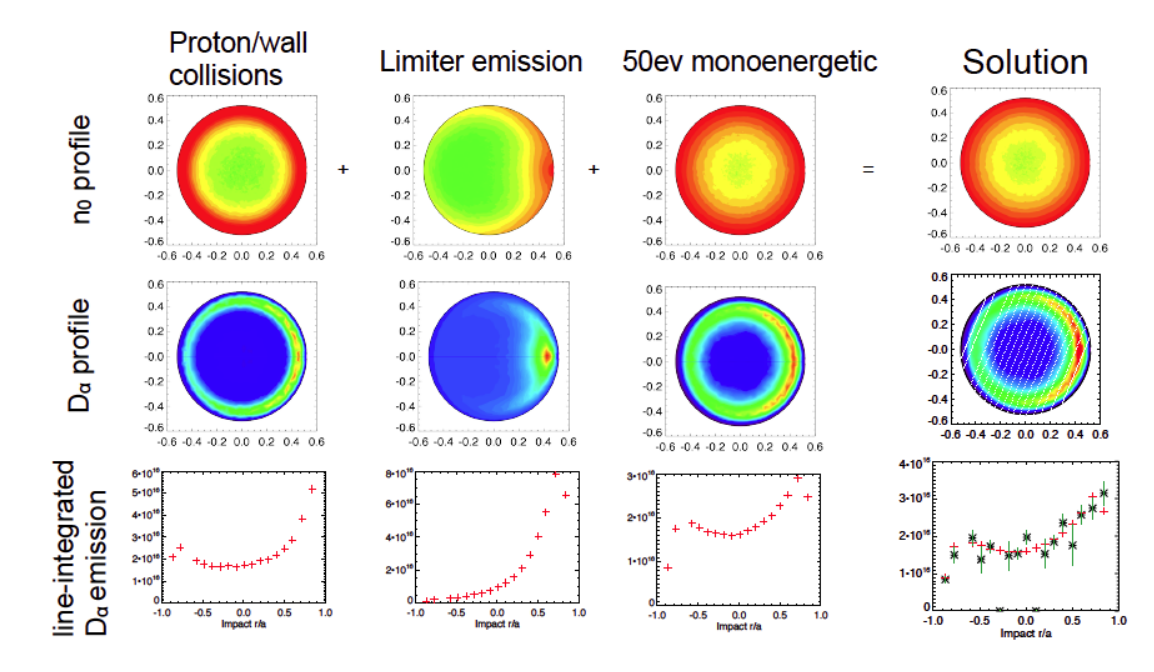
\includegraphics[width = 1.\linewidth]{ion_transport_results/nene_example.png}
	\caption[Example of NENE neutral output]{Example of NENE neutral output, the difference between this and the DEGAS2 results are examined in this section. (Reproduced from S. Eilerman's Thesis \cite{Eilerman})}\label{fig:nene_example}
\end{figure}

\subsection{Neutral source geometry, and fitting of observations}\label{sec:neutral_source_geometry}

In an ideal situation the neutral source rates would be known through direct observation and be modelled using the complete 3D geometry of the vacuum vessel. But as a practical matter, neutral recycling is complex and not within the scope of this work. Instead, a 2D neutral simulation is run with several independent neutral source profiles assuming toroidal symmetry. Each particle source has a defined geometry and rate. An instance of neutral analysis is simulated implementing each particle source independently, and then the rates are linearly fit to the observed $\dal$ emission levels (discussed in detail in section \ref{sec:DEGAS2}). Increasing the number of independent 'sources' via subdividing the wall geometry would give more fitting parameters, but the fitting problem becomes under constrained by the emission measurements, and the computational time needed increases unnecessarily. This work uses a three-source geometry as follows (illustrated in figure \ref{fig:DEGAS2_sources_and_density}):
\begin{figure}
	\centering
	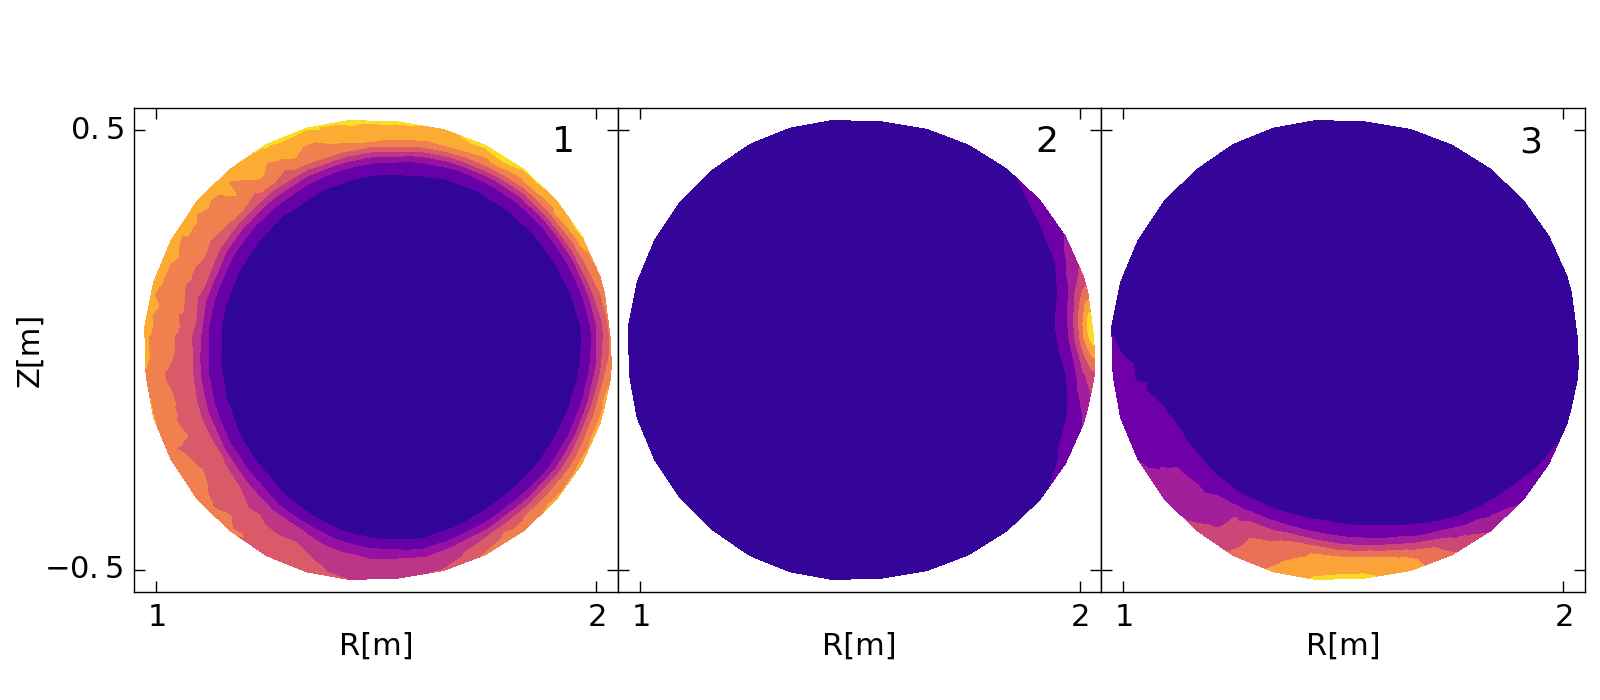
\includegraphics[width = 1.\linewidth]{ion_transport_results/source_comp.png}
	\caption[DEGAS2 source contributions]{Geometry of the normalized neutral density for the 3 sources used in DEGAS2. 1: 'Wall' source, 2:Limiter source, and 3: 'Duct' source. Details in text. It is interesting to point out that in the contribution from the 'uniform' source, there can be clearly observed the effect of the Shafronov shift on the neutral density. \textit{ie.} the neutral density 'hole' is correspondingly shifted to reflect the shift in the ionization region. This phenomenon is not seen in NENE results of the same source (figure \ref{fig:nene_example}), and it is unclear why. Though likely related to self-consistency issues in implementation.}\label{fig:DEGAS2_sources_contrib}
\end{figure}
\begin{enumerate}
    \item A poloidally uniform source representing the walls of MST, with the exception of the area detailed in the following source. 
    \item A poloidally localized source corresponding to the location of the outboard limiter. The outboard limiter (typically) defines the LCFS on MST and is known to be a major source of recycling as well as impurities.  
    \item A poloidally localized source corresponding to the bottom 45\textdegree of the wall. This is the location of the pumping duct and gas injection valves of MST. 
\end{enumerate}
The contributions from each source (to density, for example) are treated as linearly independent. This is due to the fact that neutral-neutral collisions are very rare compared with neutral-ion and neutral-electron collisions at typical parameters. Typical contributions from each source are shown in figure \ref{fig:DEGAS2_sources_contrib}. This project began by considering only the first two sources, with the second extending uniformly around the circumference of the vessel poloidal cross section. However, it is found that in some instances the first two source terms could not be used to explain measurements from the $D_\alpha$ array. In particular, the intensity on the central view chords would be systematically under-predicted by the code. By hypothesizing that the neutral population may have a vertical asymmetry due to preferential sources and sinks in the lower region of the vessel. This is the location of the pumping duct and all of the fueling gas injection valves. If this region has a different effective source rate than 'the rest of the wall', the code is then able to give a better fit to the observations. (see figure \ref{fig:DEGAS2_source_comp})%, and \ref{fig:DEGAS2_typical_fit}). Additionally, it is useful to point out that

\begin{figure}
	\centering
	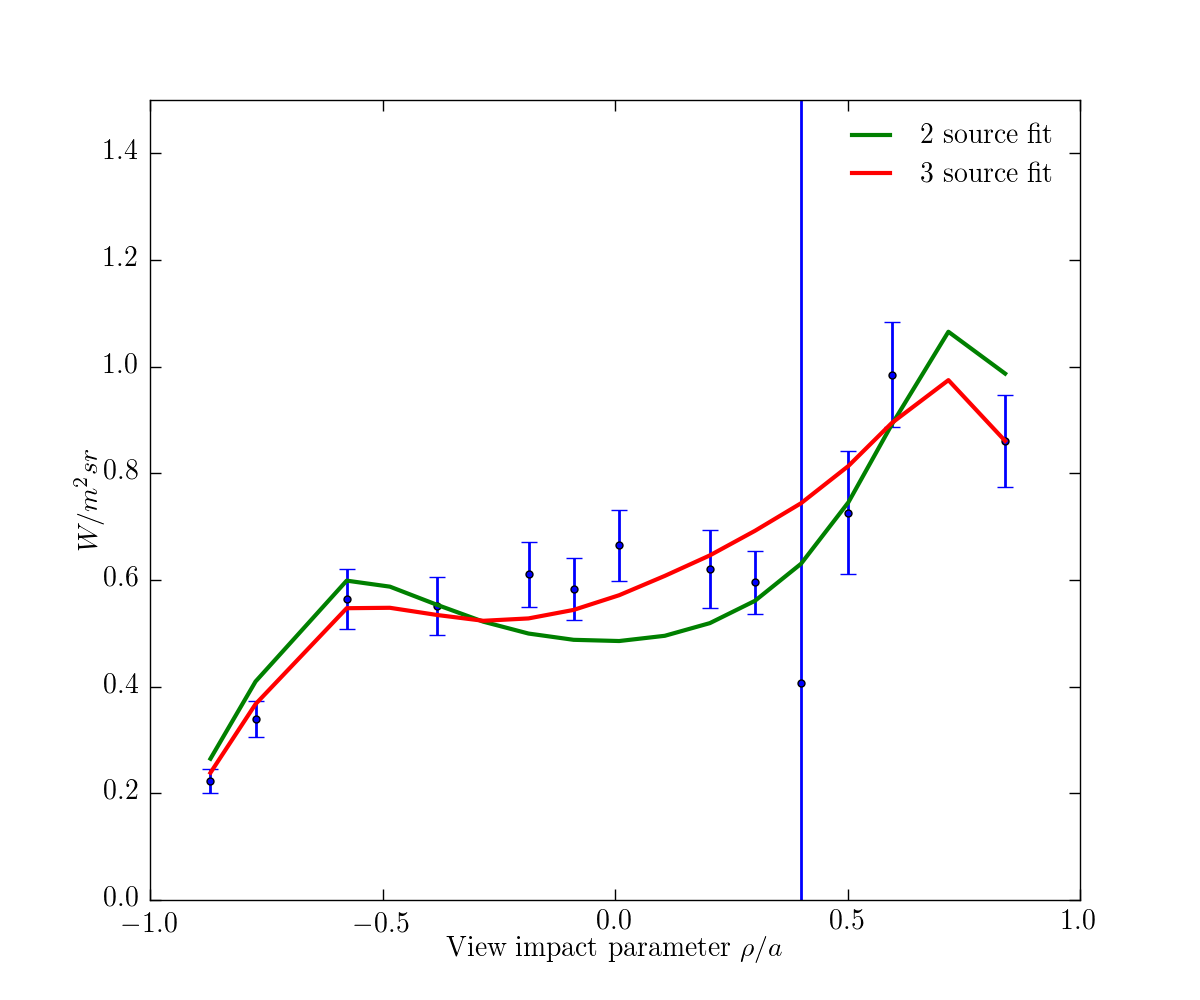
\includegraphics{ion_transport_results/source_comparison.png}
	\caption[Comparison between 2 source and 3 source fit for DEGAS2]{Comparison between 2 source and 3 source fit for DEGAS2.}\label{fig:DEGAS2_source_comp}
\end{figure}

\begin{figure}
    \centering
    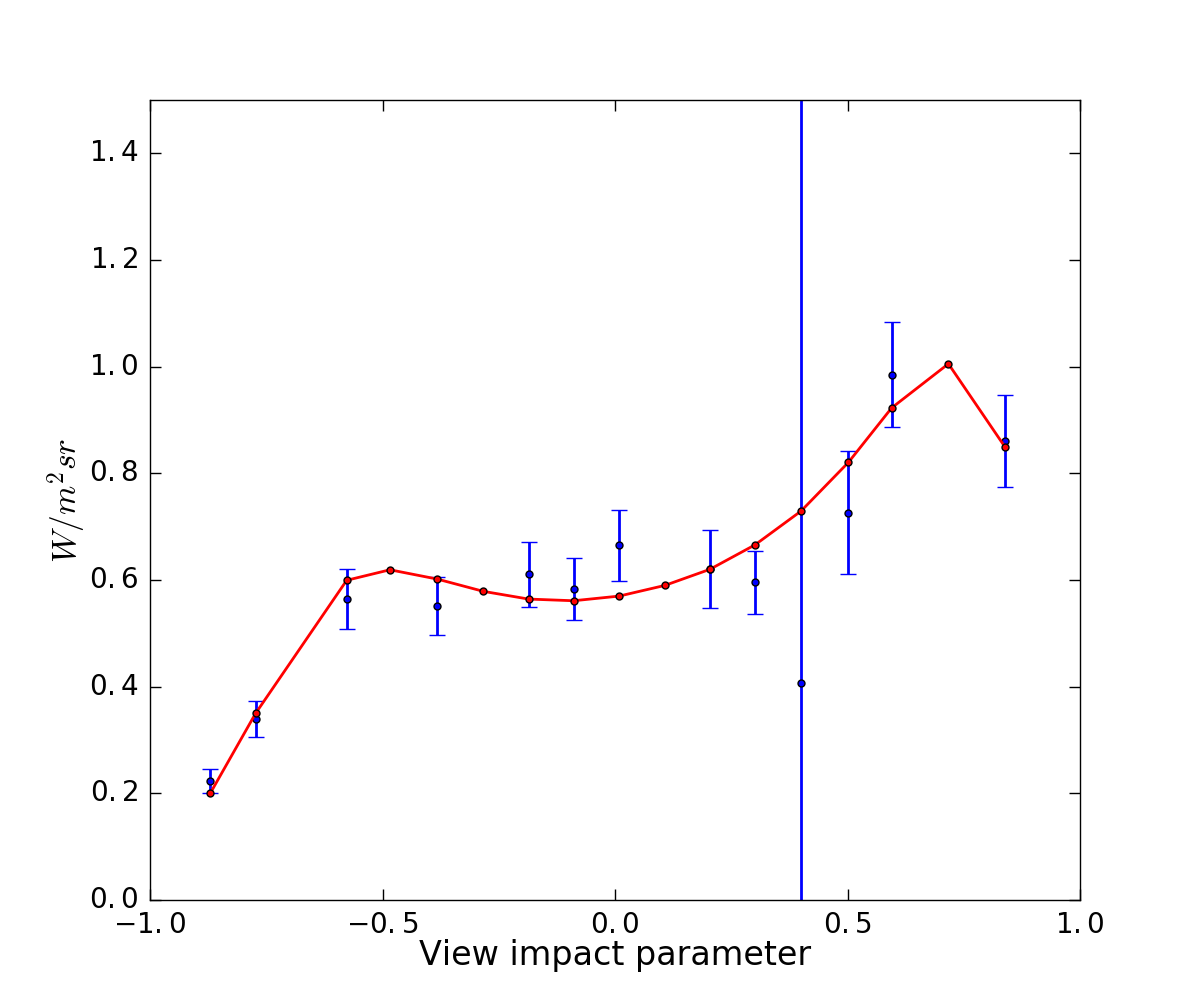
\includegraphics{ion_transport_results/DEGAS2_typical_fit.png}
    \caption{A typical DEGAS2 fit of ensembled $\dal$ signal.}
    \label{fig:DEGAS2_typical_fit}
\end{figure}

\subsection{Neutral density in PPCD}

\begin{figure}
    \centering
    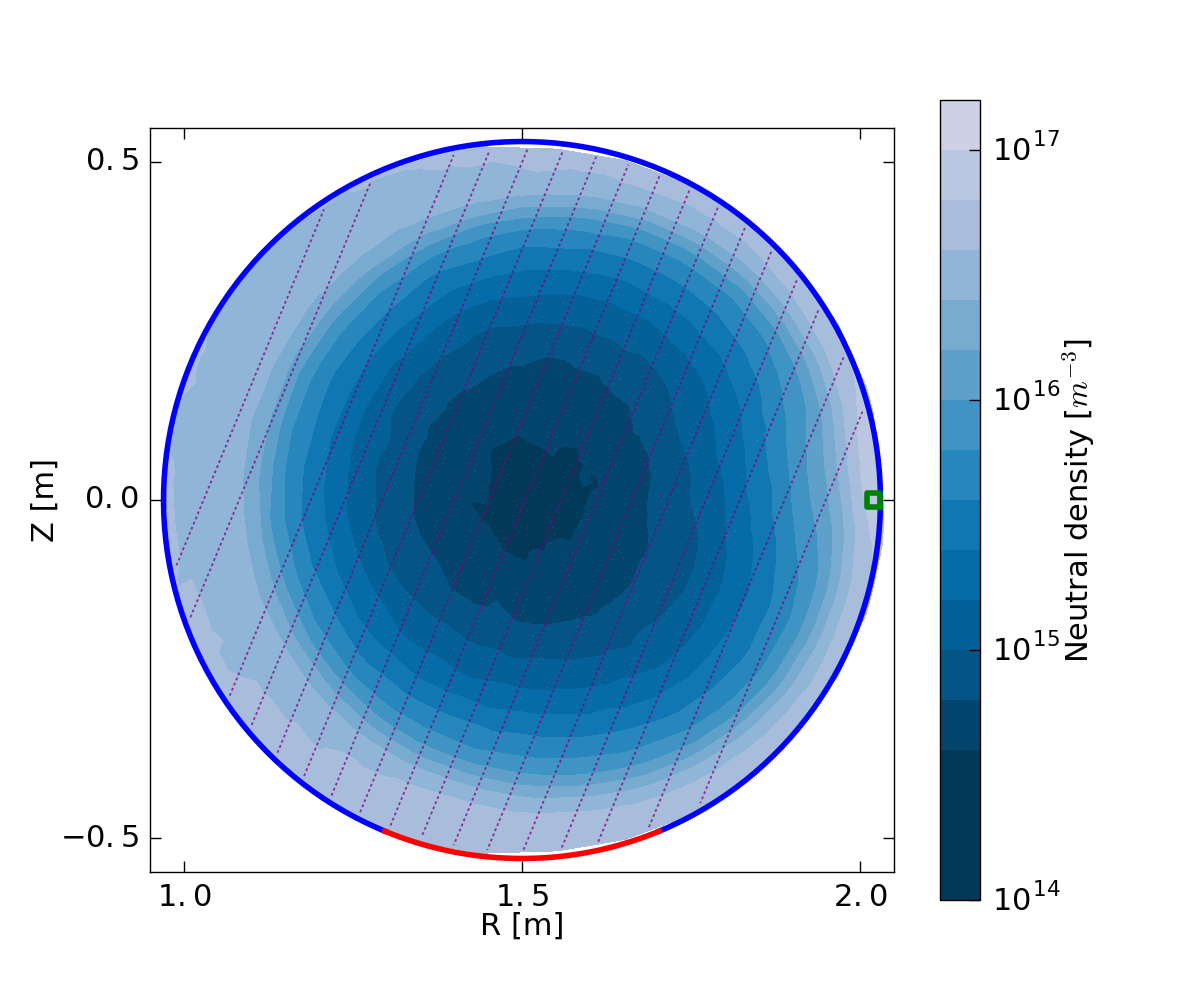
\includegraphics{ion_transport_results/DEGAS2_density2d.png}
    \caption[Neutral density via DEGAS2]{Neutral density via DEGAS2 simulation, with the geometry of the three sources overlayed. Using the numbering presented in section \ref{sec:neutral_source_geometry}: source 1 is in blue, source 2 is in green, and source 3 is in red. The dashed lines represent the location of the available views.}
    \label{fig:DEGAS2_sources_and_density}
\end{figure}

\begin{figure}
    \centering
    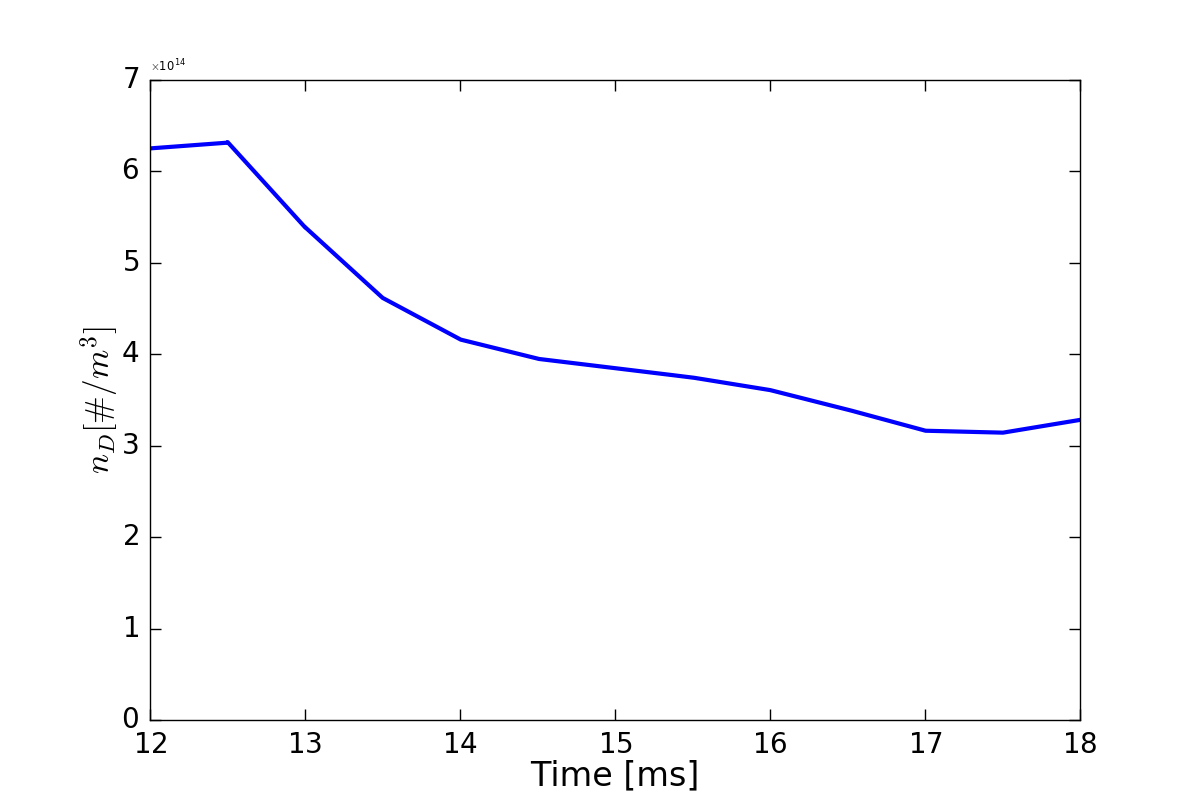
\includegraphics[width=0.8\linewidth]{ion_transport_results/neutral_vs_time.png}
    \caption[Core neutral density over time]{Core neutral density over the time span of the PPCD period. This result is from the ensemble of good PPCD shots analyzed.}
    \label{fig:neutral_vs_time}
\end{figure}

Unsurprisingly, the neutral density is edge dominated and decreases by about 2.5 orders of magnitudes as one 'travels' towards the core. The details can be seen in figure \ref{fig:DEGAS2_sources_and_density} and \ref{fig:DEGAS2_1d}. The edge neutral density is comparable with previous estimates, but the core density is about 1/4 of previous calculations using the NENE code~\cite{Eilerman2010}. % This comparison of the NENE and DEGAS2 code predictions for neutral density profiles that best fit observed neutral emission measurements doesn't really explain which model is more believable. Aside from the ad-hoc 50eV source, what are the differences between the two codes? 
%Added more on the improvement DEGAS2 makes in first paragraph of section. -Xing
Though when NENE is run for my particular shot ensemble, it returns results lower than that presented, and the core density from DEGAS2 is ~ 55\% of NENE. As pointed out above, the DEGAS2 fit have the advantage of not relying on an \textit{ad hoc} 50eV neutral source to achieve the fit, and the neutral density more self consistently show the effect of the Shafronov shift (see also figure \ref{fig:DEGAS2_sources_contrib}). 
Further, the neutral density in PPCD is not entirely constant; the early part of PPCD sees the neutral density decreasing until around 16.5ms when it stabilizes until the end of PPCD (figure \ref{fig:neutral_vs_time}. This neutral density estimates is also in line with that from s. Kumar's measurement of Al charge state fractions in the core. The charge state fraction of Al$^{11+}$ to Al$^{13+}$ is very sensitive to neutral density as the charge exchange process keep the Al$^{13+}$ population down. DEGAS2's estimate of core neutral density. The DEGAS2 neutral density is still too might to match that needed by J. Waksman to explain the NBI heating effects observed. However, this is perhaps not a good direct comparison as his work are on well optimized low current (200kA) PPCD, which, other than the problem of differing plasma current as my parameters, is inherently difficult for $\dal$ observations to constrain neutral density as the emission measurements begin to approach noise levels of the detector. 

\begin{figure}
    \centering
    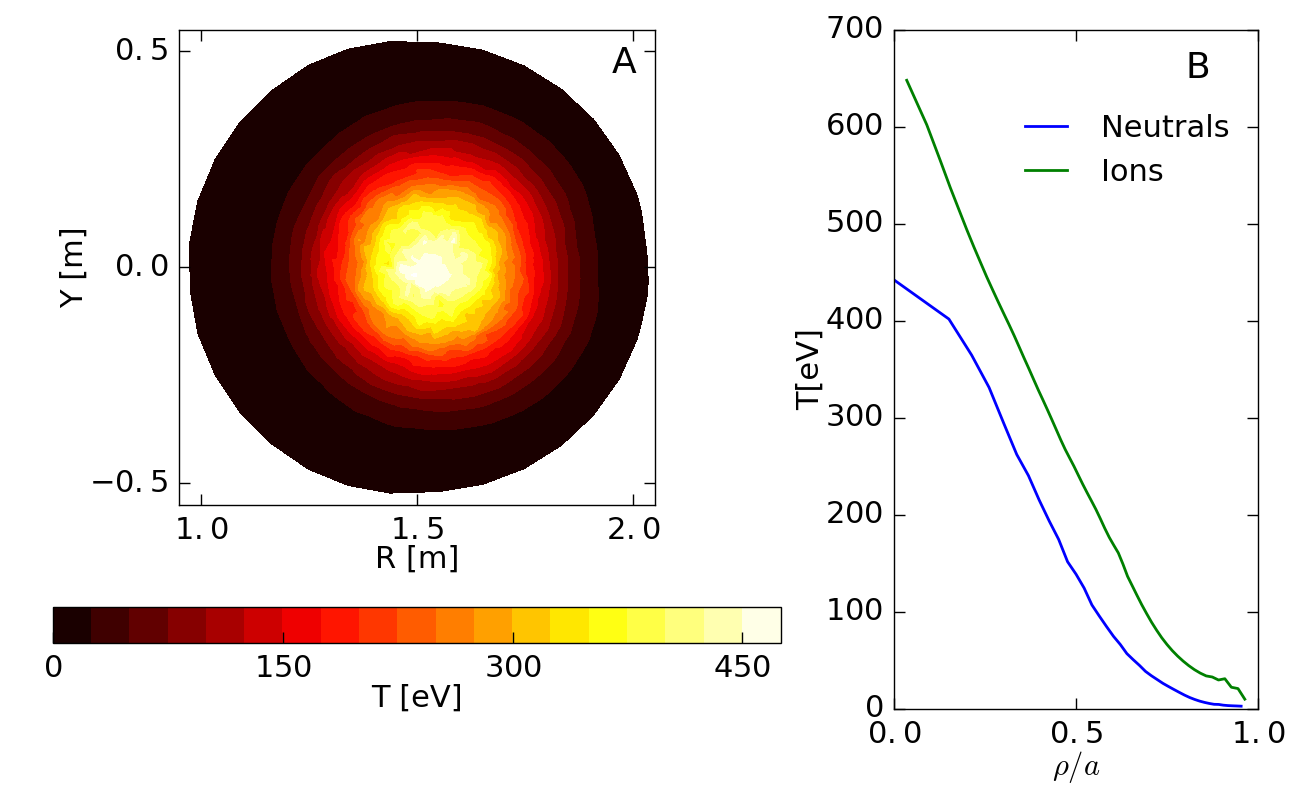
\includegraphics[width=\linewidth]{ion_transport_results/DEGAS2_temperature2d.png}
    \caption[Neutral temperature via DEGAS2]{Neutral temperature via DEGAS2 simulation. A) The 2-d temperature results. B) The flux surface averaged results, with $T_i$ for comparison.}
    \label{fig:DEGAS2_temperature}
\end{figure}

Another notable improvement of the understanding of the neutral dynamics is the neutral temperature information provided by DEGAS2. Though it may not be immediately obvious, but a high $T_{\text{neutral}}$ is needed for the neutrals to penetrate into the plasma volume. The mean free path of a 'room temperature' neutral is very short in MST parameters, and neutrals created by charge exchange reactions, and a small amount of Frank-Condon neutrals from energetic disassociation of D$_2$ would dominate the neutrals interior to the plasma. This is reflected by the DEGAS2 results (figure \ref{fig:DEGAS2_temperature}). Notably, the neutral temperature is a significant fraction of the ion temperature, meaning that only a fraction of the ion's thermal energy is effectively lost in a charge exchange reaction.

\subsection{Charge exchange, impact ionization, and ion source rate}

\begin{figure}
    \centering
    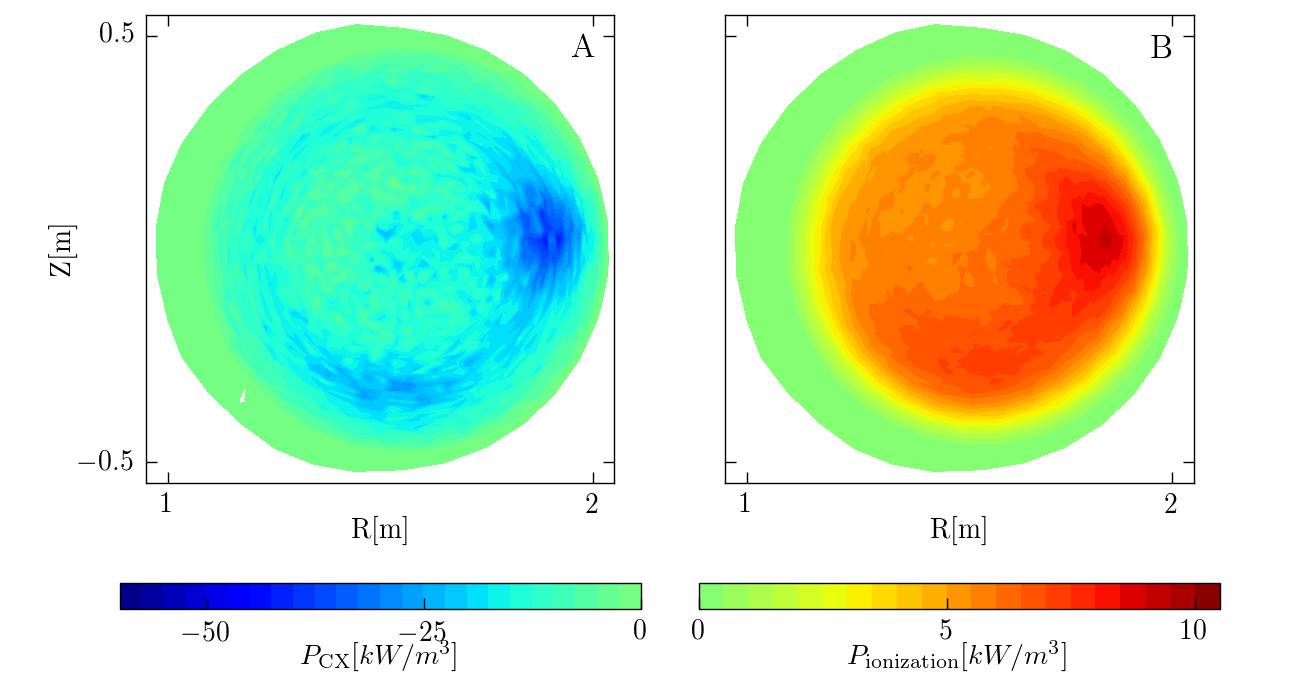
\includegraphics[width=\linewidth]{ion_transport_results/DEGAS2_power_terms_2d.png}
    \caption{DEGAS2 2D  A) charge exchange and B) impact ionization terms. Note the difference in the color bar range. Less obviously, the up/down asymmetry is also present in this plot. This result is from ensembled PPCD shots at 15ms.}
    \label{fig:DEGAS2_power_2d}
\end{figure}

\begin{figure}
    \centering
    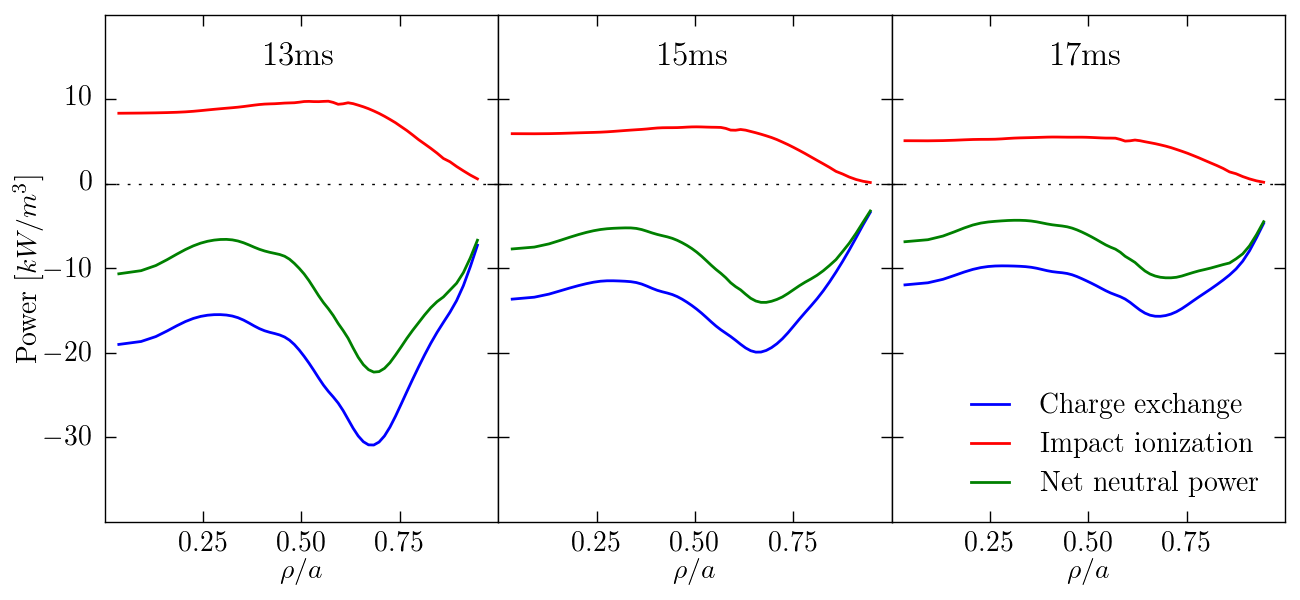
\includegraphics{ion_transport_results/DEGAS2_power_terms_1d.png}
    \caption{1-D neutral power terms at 13ms, 15ms, and 17ms. The 'net neutral power' refers to the sum of the two terms, as electron impact ionization is a process that recovers some thermal energy from the neutrals fluid.}
    %This plot should include 'net charge exchange loss'
    \label{fig:DEGAS2_power_1d}
\end{figure}


The charge exchange loss rate displays an hollow profile that is significantly skewed outboard, like the ion density. However, the poloidal transit time are small on the RFP and neutral effect on the majority ion fluid is still considered on a flux surface averaged basis despite significant asymmetry. On a practical basis, this hollow profile is the creation of the declining neutral density towards the core, and the increasing majority density as well as temperature difference. The trend of declining neutral density also translates to the charge exchange loss as expected. The electron impact heating is an interesting to consider as it represents a partial 'recovery' of the thermal energy lost in charge exchange (details in section \ref{sec:neutral_physics}). However, as the neutral's temperature is below that of majority ion, this actually results in temperature decrease. In general, I use 'heating' to describe thermal energy input into the ion fluid which does not necessarily increase the temperature. 

\begin{figure}
    \centering
    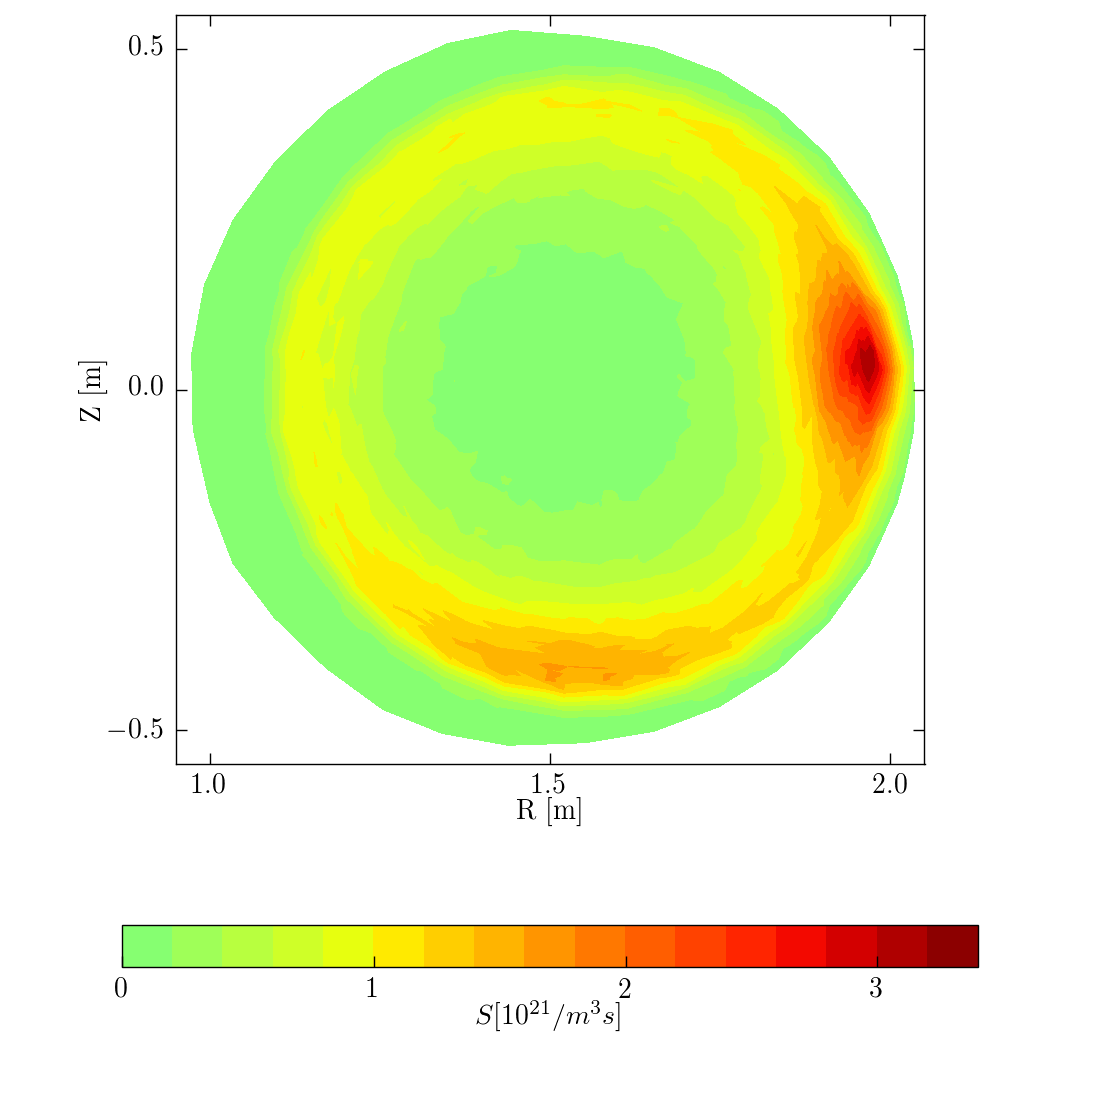
\includegraphics{ion_transport_results/source_2d.png}
    \caption{DEGAS2 ion source rate results.}
    \label{fig:DEGAS2_source_rate}
\end{figure}

The ion source rate also displays the same characteristics as the power terms. However, it is significantly more hollowed out since it does not depend on the difference in ion and neutral temperature, which is higher in the core. This means that the ion source rate is not sufficient to explain the density rise in the core. The consequence of this is to hint at an inward pinch mechanism to be explained in more detail in section \ref{sec:eb_pinch}

%\subsection{Unintuitive model response of \textit{ad hoc} heating in the edge}
%\begin{figure}
%    \centering
%    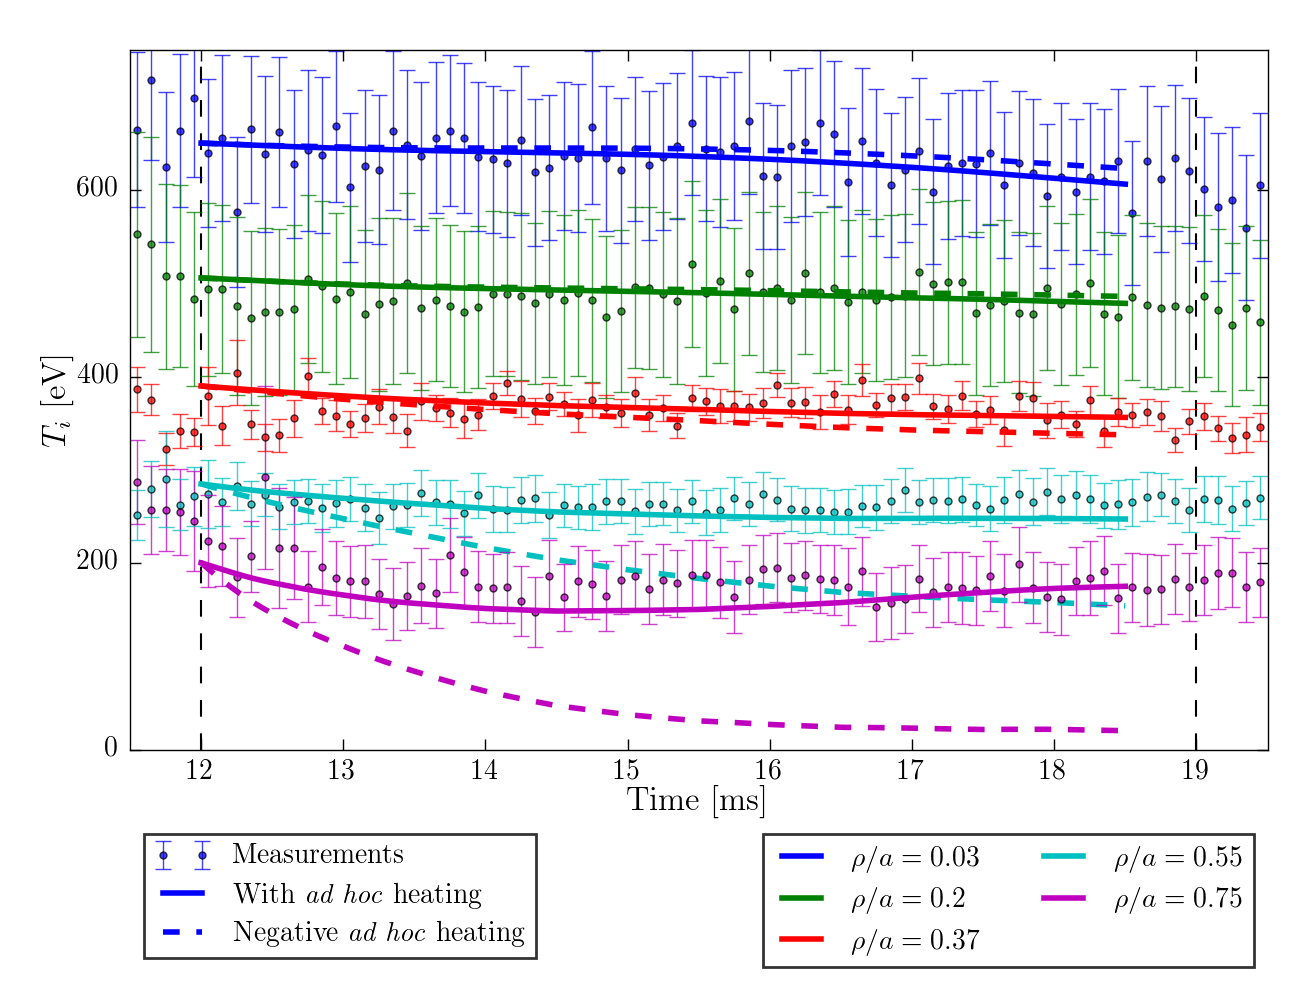
\includegraphics[width=\linewidth]{ion_transport_results/unintuitive_response.png}
%    \caption{The effect of having a low ion temperature edge on charge exchange}
%    \label{fig:unintuitive_cx_response}
%\end{figure}

%During the adjustment process for the model, it became clear that ion heating in the edge have an effect on the charge exchange loss in the core through it's effect on ion temperature. Suppose you have an edge region where the ion temperature is only a few eVs, but the electrons are on the order of 50 to 100 eV. In this region, electron impact ionization of neutrals would dominate charge exchange, and any neutral particle entering the plasma would more likely be ionized before undergoing charge exchange, thus decreasing the neutral penetration. The decreased penetration would in turns result in a more hollowed out neutral density, as well as charge exchange loss and ion source rate. This situation was created in the model from a mistake in the calculation in the flow effects in the edge, and when \textit{ad hoc} heating is applied this erroneous model to bring it inline with the observed temperature without changing how the rest of the model is calculated, the core temperature is predicted to be lower. However, this effect seems most significant when the edge ion temperature drops to ~10eV or lower for a significant radius. When the mistake was corrected, the model predicted edge ion temperature of ~50eV at $\rho_v/a \approx 0.75$ without \textit{ad hoc} heating terms, and increasing it to the observed ~175eV using \textit{ad hoc} heating only dropped the core temperature very slightly.


\section{Pinch in the Reverse Field Pinch}\label{sec:eb_pinch}
%\section{Observations of inward pinch flow associated with $\vec{E}\times\vec{B}$ drift and it's effect on ion thermal transport}

%In previous power balance work, the heat lost to particle flow is one of the largest terms\cite{Fiksel2006}. Calculating $P_{flow}$ involves estimating the ion particle flux.  However, no diagnostic measurements of $n_i$ in MST is available, therefore, $n_i$ is inferred indirectly through the evolution of $n_e$ combined with previous work on characterizing the impurity content in PPCD\cite{Kumar2012,Nornberg2018IncorporatingCharge}.

%...

%Given that the  calculated electron source rates are insufficient to account for the density rise, another possibility is an inward particle flux. The particle flux ($\Gamma_{obs}$) needed to satisfy the continuity equation (\ref{eqn:cont}) is then calculated. However, we seek to confirm the theoretical plausibility of an inward pinch by considering the evolution of the magnetic equilibrium.

%There is currently no diagnostic that measures the poloidal and toroidal $\vec{E}$, which is needed to constrain the radial $\Gamma_{\vec{E}\times\vec{B}}$. Instead, the slow time-scale E field is estimated using the evolution of reconstructed B field from edge flux coil and FIR polarimetry data. The radial flux, $\Gamma_{\rho} = n_e\frac{(\Vec{E}\times\Vec{B})_{\rho}}{B^2}$, is constrained by $E_{pol}$ and $E_{tor}$. The MSTfit equilibrium reconstruction outputs reconstructed flux values and flux surfaces in 2D which enables the calculation of $E_{pol}$ and $E_{tor}$. In particular $E_{pol}$ can be calculated through:

%\begin{align}
%   E_{pol}(\rho_v) & = -\frac{1}{\rho_v}\int_{0}^{\rho_v}\rho_v' \frac{dB_{tor}}{dt} d\rho_v'
%\end{align}

%where it is taken as a boundary condition that the $E_{pol}$ is zero at the magnetic axis.

%where $\rho_v$ is the flux surface averaged minor radius.

%Calculating $E_{tor}$ is slightly more complicated, as it is a function of major radius and not $\rho$. On MST, there is a poloidal gap (a cut in the vessel in the poloidal plane) in the conducting wall and the voltage measured across the gap ($V_{PG}$) is a reflection of the inductively driven toriodal E field. To incorporate into the 1-D approximation, $E_{tor}(R, Z=0)$ along the Z = 0 plane is determined as a function of major radius (R) through:

%\begin{align}
%\oint_S \vec{E}\cdot d\vec{l} &= -\iint \frac{\partial}{\partial t}\vec{B}\cdot d\vec{s}\\
%E_{tor}(R) 2\pi R &= -\int_0^{2\pi}\int_{R_{in}}^{R}R'\frac{\partial B_{pol}}{\partial t} d\phi'dR' - V_{PG}\\
%E_{tor}(R) &= -\frac{1}{R}\int_{R_{in}}^{R}R'\frac{\partial B_{pol}}{\partial t} dR' - \frac{V_{PG}}{2\pi R}\label{eqn:E_tor}
%\end{align}
%where $R$ refers to the major radius, and $R_{in}$ is the major radius at the inboard wall.

%Since the $ \frac{dB}{dt} $ term cannot be evaluated directly, sequential MSTfit reconstructions, 0.5ms apart are used to provide $ B_{pol} $ and $ B_{tor} $ information from which a numerical derivative is calculated. The results show $E_{tor}$ to be relatively stable in the core, but changes direction in the edge as time progresses. This reversal correlates with current drive being exhausted in the edge. Note this is not related to the edge $\vec{B}$ reversal that gives the RFP it's name. From $E_{pol}$ and $E_{tor}$, the radial particle flux is calculated as: 

%\begin{equation}
%\Gamma_{\vec{E} \times \vec{B}} = n_{e} \frac{E_{pol}B_{tor} - E_{tor}B_{pol}}{B^2}
%\end{equation}

%and this is compared to $\Gamma_{obs}$ previously calculated from Eqn. \ref{eqn:cont} and shown in Fig. \ref{fig:flux_compare}. From the core to about the mid radius, the estimated $\Gamma_{\vec{E} \times \vec{B}}$ tracks the flux needed to account for density change well. However, further into the edge, there is residual flow outwards since the neutral ionization rates are faster than density growth, thus particle loss is need to balance the continuity equation. This is likely caused by transport mechanisms such as turbulence due to drift wave activity\cite{Duff2018ObservationPlasmas,Williams2017TurbulencePinch,NishizawaPRLSubmitted}. Importantly, the $ E_{tor} $ reversal during the PPCD period causes the estimated $ \Gamma_{\vec{E} \times \vec{B}} $ flow to cease. This echoes MHD calculations by J. Reynolds that found the $ E \times B $ flow would cease as the axial E field is reduced and reversed\cite{ReynoldsThesis}.

%Using $\Gamma_{obs}$, the flow contribution to heat balance is calculated using Eqn.\ref{eqn:flux_terms} and found to be the largest term in the core of the plasma (Fig. \ref{fig:dedt_plot}). Breaking it down further, the notable observation is that the compression heating is larger than the equlibration heating and is the largest heating term in the core. The conservation term is larger, but does not cause temperature to rise as it represents the thermal energy carried by the particle inflow. The temperature in the core is predicted to rise slightly while in the gradient region it would decrease as the colder ions flow in.
As mentioned in the previous section, the ionization rates in the core are insufficient to account for the electron density increase observed. Additionally, the impurity contribution to the electron density rise is small in order of magnitude compared with what is 'needed'. This presents a dilemma for the model since quasi-neutrality dictates that the ion density rise with that of electron, but if a source for this 'extra' density is to be assumed, then the temperature of this ion source is also to be assumed. From a ion thermal modeling point of view, allowing an arbitrary temperature to be associated with an anomalous density term is problematic as it can be a large thermal term compared to the other mechanisms, and allowing it to be adjusted at will on the researcher's (my) whim weakens the validity of the model. It would be much preferable for the mechanism to be discovered instead being assumed. 

\begin{figure}
    \centering
    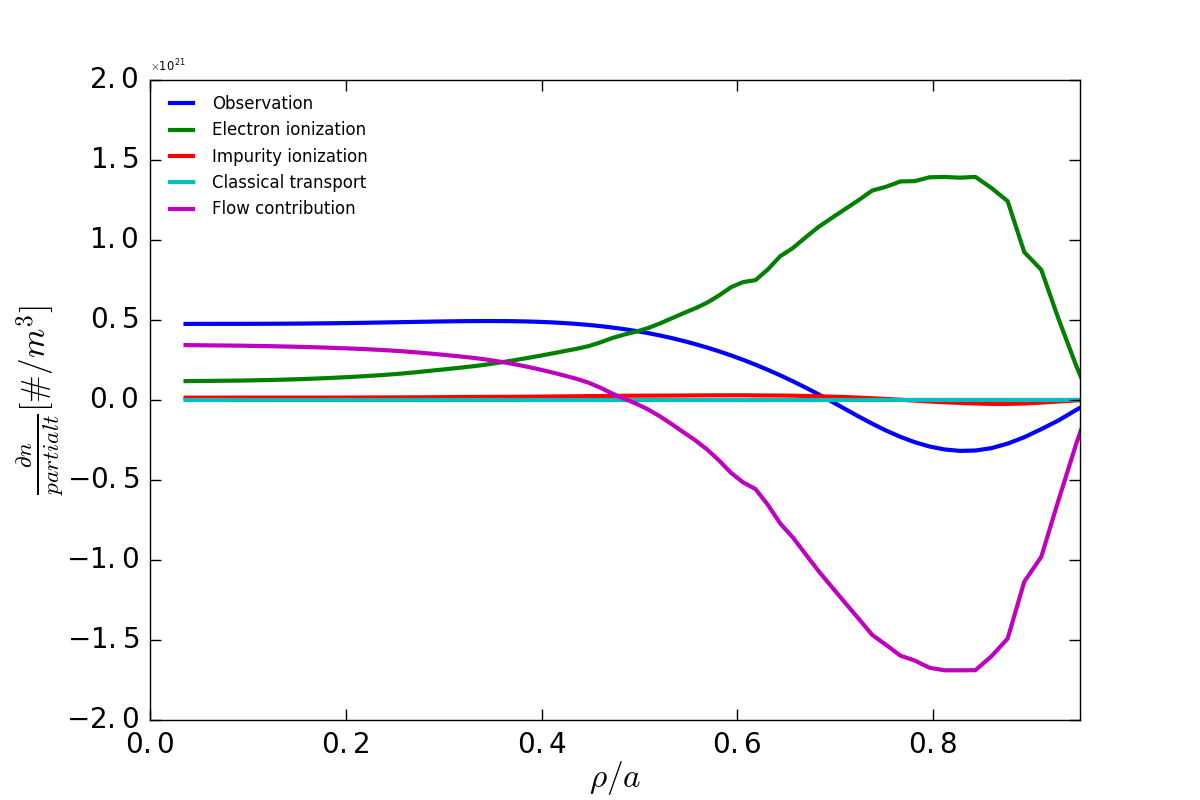
\includegraphics{ion_transport_results/density_balance.png}
    \caption{$\partialt n_e$ in MST and their sources. This particular plot presents the ensembled analysis at 14ms.}
    \label{fig:density_balance}
    %%TODO, need larger legend text.
\end{figure}

The first step is realizing that source rate mechanisms are limited. Ionization of deuterium and impurities accounts for all the available sources of electrons. However, particle flow has not been explored to the same degree. In J. Reynolds's thesis on simulating the effect of PPCD using the numerical MHD code NIMROD \cite{Reynolds2007}, he observes the simulation undergoing an inward pinch flow across the simulated plasma volume (see figure \ref{fig:NIMROD_pinch}). He also refers to previous simulation studies on PPCD-like conditions showing inward pinch\cite{StuffThatReynoldCited}. More empirical on MST, PPCD drive the plasma into deep reversal and the reversal surface moves inwards during this process. Previous measurements of electron density using FIR also show the gradient region moving inwards (figure \ref{fig:Ne_gradient_pinch}), hinting at a pinch. After all, it is in the name of the configuration.

\begin{figure}
    \centering
    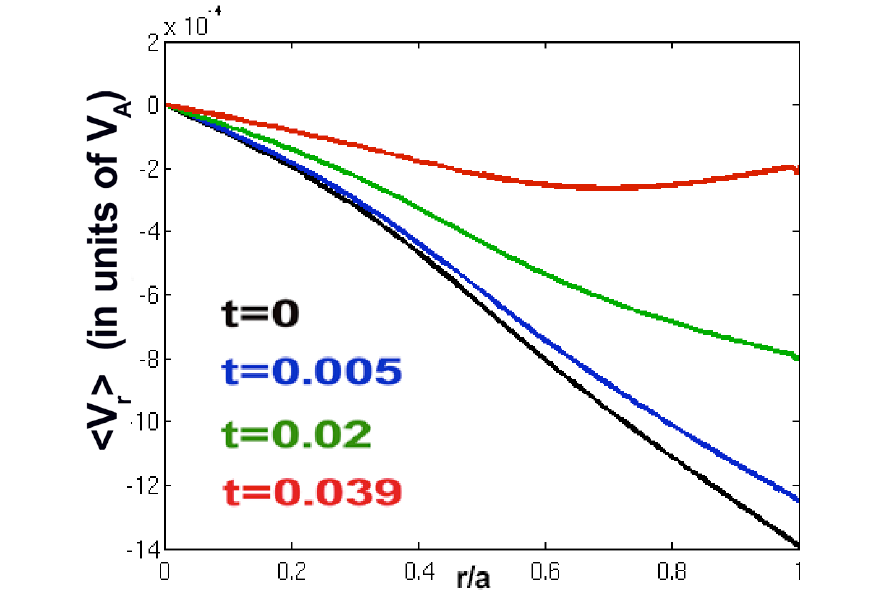
\includegraphics{ion_transport_results/reynold_pinch.png}
    \caption{Pinch velocity from J. Reynolds' simulations. Note that the simulation volume ends at the reversal surface and the Lunquist number of the simulation is lower than actual plasma conditions. (Reproduced from J. Reynolds\cite{ReynoldsThesis}). }
    \label{fig:NIMROD_pinch}
\end{figure}


Working with the hypothesis that the unaccounted for core density rise is due to a pinch flow, I use the continuity equation (equation \ref{eqn:continuity}) to calculate the particle flux needed to balance out the observations. This forms a basis for comparison with the hypothesized mechanism, \ecb drift.

\subsection{Estimating radial \ecb drift}

MST have limited ability to diagnose $\vec{E}$ field in high current plasmas. Thus the $\vec{E}$ needs to be estimated from indirectly from the $\partialt\vec{B}$ according to the Maxwell equations. The $\vec{B}$ field are calculated by the equilibrium reconstruction code MSTfit using inputs from the gap voltage measurements, edge pick up coils, and FIR polarimeter measurements. Sequential MSTfit equilibrium reconstruction are used to estimated $\partialt\vec{B}$. From there $E_{pol}$ can be calculated through:
\begin{align}
   E_{pol}(\rho_v) & = -\frac{1}{\rho_v}\int_{0}^{\rho_v}\rho_v' \frac{dB_{tor}}{dt} d\rho_v'
\end{align}
where it is taken as a boundary condition that the $E_{pol}$ is zero at the magnetic axis.

The calculation of $E_{tor}$ is slightly more complicated, as it is a function of major radius and not $\rho_v$. The voltage measurement ($V_{PG}$) across the poloidal gap on MST (a cut in the vacuum vessel along its intersection with the poloidal plane) is a reflection of the toriodal E field at the wall and serves as the boundary condition for the integration. $E_{tor}(R, Z=0)$ along the Z = 0 plane is determined as a function of major radius (R) through:
\begin{align}
\oint_S \vec{E}\cdot d\vec{l} &= -\iint \frac{\partial}{\partial t}\vec{B}\cdot d\vec{s}\\
E_{tor}(R) 2\pi R &= -\int_0^{2\pi}\int_{R_{in}}^{R}R'\frac{\partial B_{pol}}{\partial t} d\phi'dR' - V_{PG}\\
E_{tor}(R) &= -\frac{1}{R}\int_{R_{in}}^{R}R'\frac{\partial B_{pol}}{\partial t} dR' - \frac{V_{PG}}{2\pi R}\label{eqn:E_tor}
\end{align}
where $R$ refers to the major radius, and $R_{in}$ is the major radius at the inboard wall. To incorporate into the 1-D approximation, the inboard and outboard $E_{tor}$ is averaged according to their flux surface subsequently. From these, we can calculate the radial \ecb flux,
\begin{align}
    \Gamma_{\vec{E} \times \vec{B}} &= n_e v_{\mecb} \nonumber \\
    &= n_{e} \frac{E_{pol}B_{tor} - E_{tor}B_{pol}}{B^2}
\end{align}
The result of this calculation is shown in figure \ref{fig:eb_v}. This can be compared with the observed flux calculated from the continuity equation (figure \ref{fig:eb_v}). The result show that \ecb is a good explanation for the inwards flow needed to balance out the observations. Hence, the $\partialt n_e$ rise in the core can now be accounted for in such a way that the associated ion temperature is no longer arbitrary, since \ecb flow is ambipolar.

\begin{figure}
    \centering
    \includegraphics{ion_transport_results/eb_v.png}
    \caption[Calculated \ecb pinch velocity]{Calculated \ecb pinch velocity. The velocity is plotted to the reversal surface. Compares well with MHD simulations results in figure \ref{fig:NIMROD_pinch} qualitatively. }
    \label{fig:eb_v}
\end{figure}
\begin{figure}
    \centering
    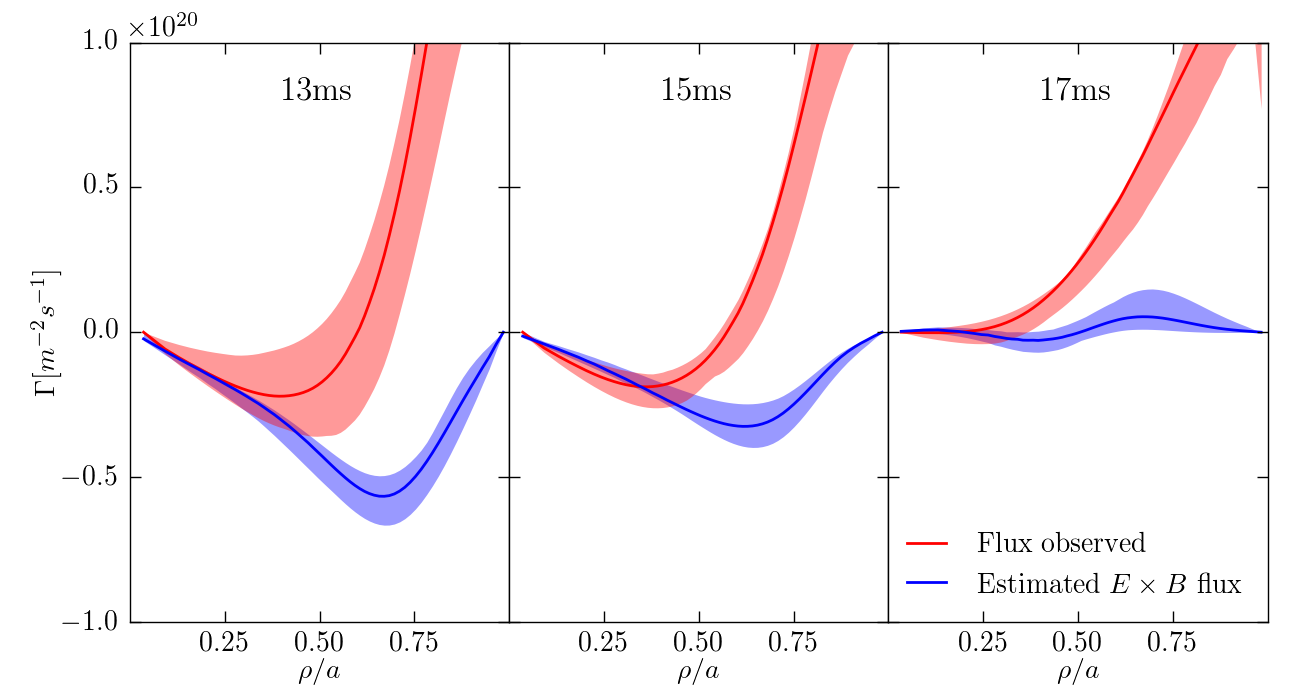
\includegraphics{ion_transport_results/flux_comp.png}
    \caption[\ecb flux compared to measured flux]{\ecb flux compared to the observed flux. 'Observed' flux is that implied by the continuity equation though $\partialt n$ and source rate observations. The two match until the mid-radius. The outer areas of the plasma is dominated by an outward anomalous particle flux. The outward flux at the edge is consistent with previous estimates\cite{TakashisSource}. }
    \label{fig:eb_v}
\end{figure}

\subsection{Flow effects on thermal transport}

The effects of the flow can be calculated via the method laid out in section \ref{sec:flow_effects}. It is useful reiterate the two components of the flow effect. One has to do with the conservation of the energy being carried by the ions. This term brings energy into the core, but generally will result in cooling, whereas it brings energy out of the edge (loss to wall), but is general increasing temperature as they are 'replaced' by ions flowing out from mid-radius. The other term is the compressional work by the \ecb drift in varying fields. This is calculated from the estimated drift velocity, and is a mostly positive term, and since it doesn't not have density effects, it represents a temperature increase. The details of these two terms are presented in figure \ref{fig:flow_power_terms}. 

\begin{figure}
    \centering
    \includegraphics{ion_transport_results/flow_power_terms.png}
    \caption[Power terms resulting from radial ion flow]{Power terms resulting from radial ion flow.}
    \label{fig:flow_power_terms}
\end{figure}

\section{Model comparison with measurements: anomalous heating in the edge.}\label{sec:results_results}
\begin{figure}
    \centering
    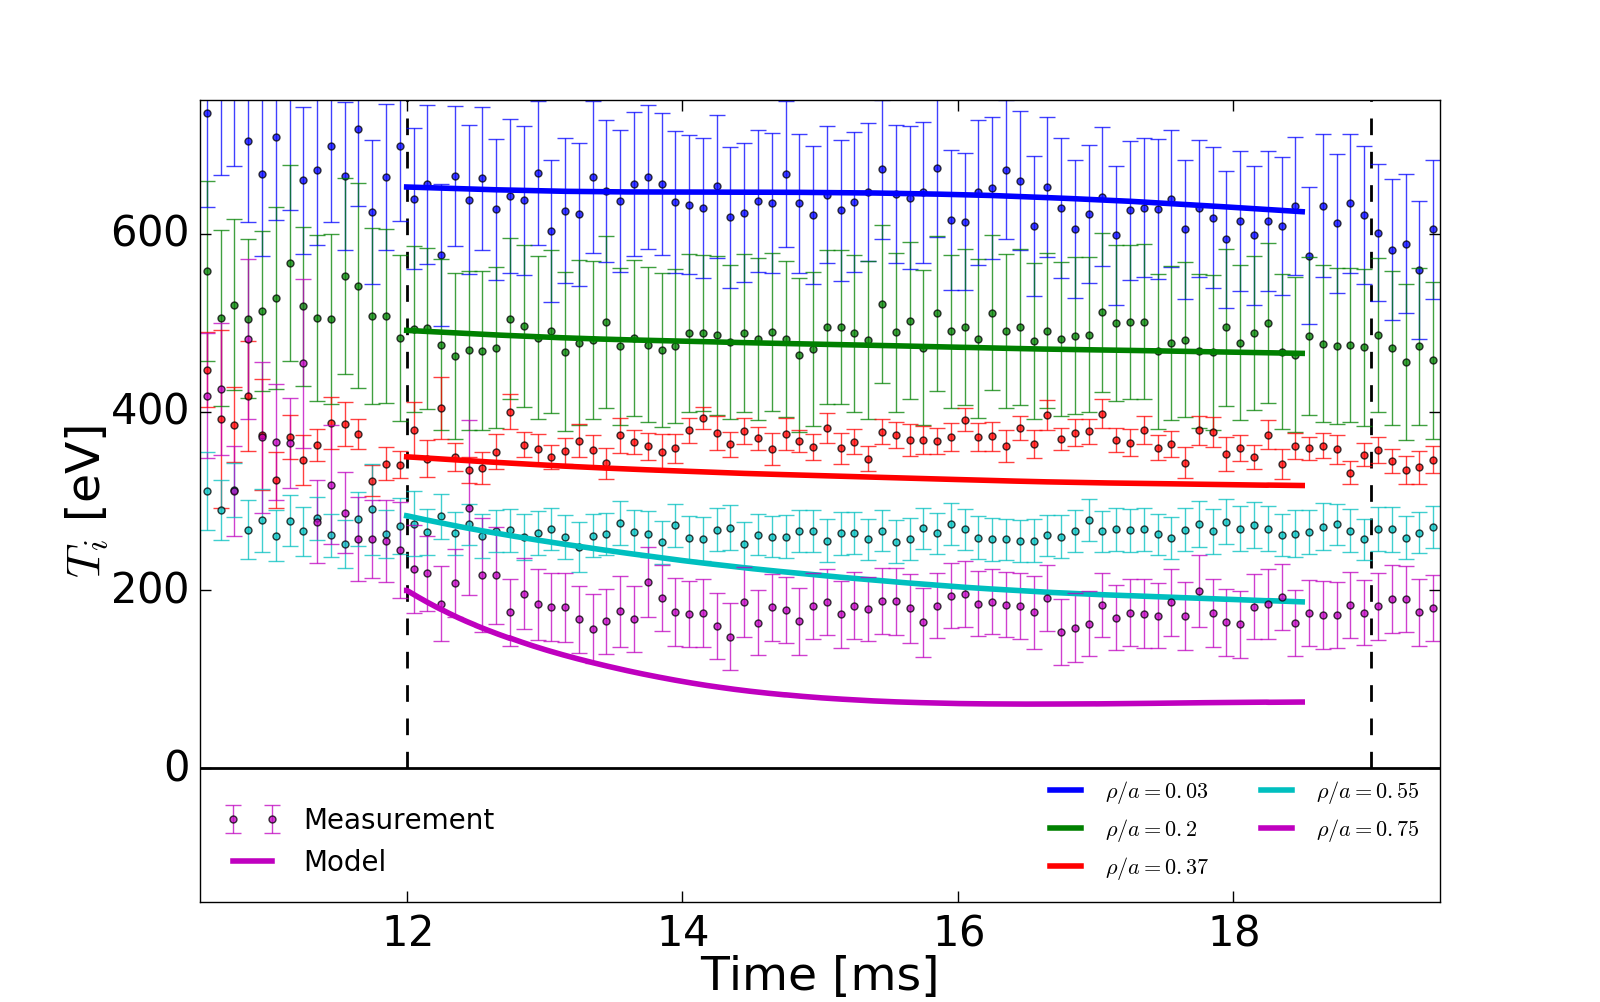
\includegraphics[width = \linewidth]{ion_transport_results/temperature_results.png}
    \caption[Temperature comparison with measurement]{Temperature comparison with measurement.}
    \label{fig:temperature_results}
\end{figure}

\begin{figure}
    \centering
    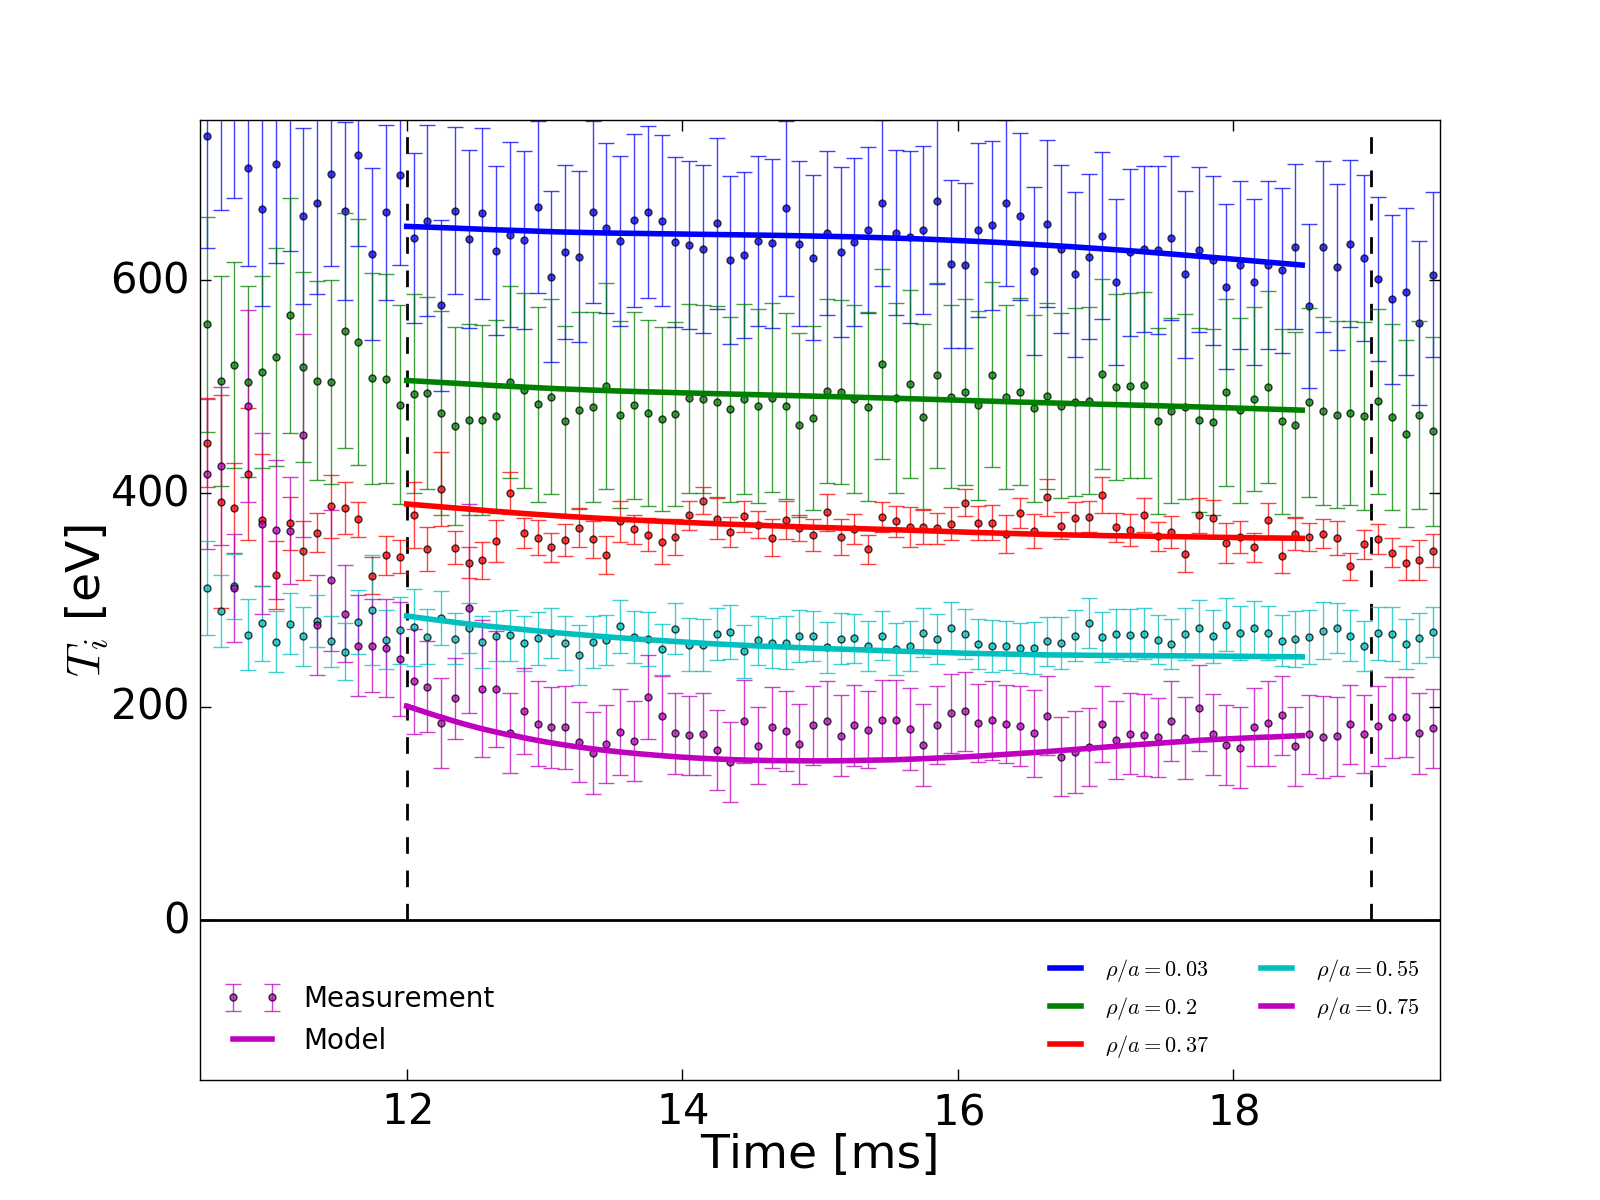
\includegraphics[width = \linewidth]{ion_transport_results/temperature_with_adhoc.png}
    \caption[Temperature comparison with measurement with \textit{ad hoc} term included]{Temperature comparison with measurement with \textit{ad hoc} term included.}
    \label{fig:temperature_results_ah}
\end{figure}

\begin{figure}
    \centering
    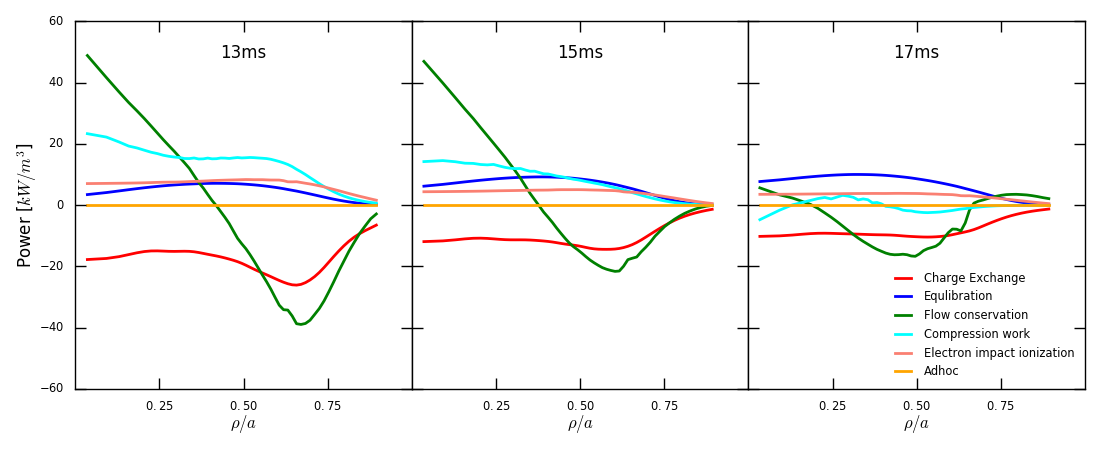
\includegraphics[width = \textwidth]{ion_transport_results/power_terms_no_adhoc.png}
    \caption[Power terms resulting from radial ion flow]{Power terms resulting from radial ion flow.}
    \label{fig:power_terms_no_ahoc}
\end{figure}
The quality of the model is evaluated by comparing its prediction to the ion temperature measurement made with CHERS. The model is initiated at 12ms, about 2ms after the first PPCD capacitor bank 'fires', as it is the earliest time when the significant suppression of tearing mode turbulence are achieved. CHERS measurement of temperature at initialization time is fit to an alpha model profile and then input into the model as initial condition. The time evolution of ion temperature is calculated according to the physics terms described in the previous sections and chapters. The model is found to adequately predict the temperature in the core, but not in the edge. To account for the edge temperature, an \textit{ad hoc} heating term is added. The model comparison results can been seen in figure \ref{fig:temperature_results}.  The most significant power loss terms (figure \ref{fig:power_terms_no_ahoc}) affecting this region is charge exchange, and thermal energy carried by particle flow (flow conservation). It is interesting to note that these loss terms are to a large extent a function of temperature as much if not more than as a function of temperature gradient. This dependence on $T_i$ is a factor that result in there being an 'equilibrium' temperature for the model. For the case where no \textit{ad hoc} heating is included, the ion temperature at near the edge would decrease until it levels off at significantly lower temperatures than the measured. In particular, figure \ref{fig:temperature_results} superficially suggest that (for the edge chord location) the temperature decreases rapidly early during the PPCD period. But initializing the model at later starting time would have the model reproduce the same behavior and settle at the same edge temperature, just now delayed. This indicates that it is not some particular circumstance relating to the early PPCD period that causes the model to under predict the temperature. But the model behaves in such a way that the edge temperature trends towards and `equilibrium' temperature determined by the power terms, which is significantly lower than the actual equilibrium temperature that the ion fluid comes to. To remedy this under prediction, an \textit{ad hoc} term is introduced into the model to raise the model's 'equilibrium'. The particular profile shape and location used for the \textit{ad hoc} term is discussed in detail in the next section, but the result of this are presented in figure \ref{fig:temperature_results} and \ref{fig:power_terms_with_adhoc}. With this addition, the model is able to account for the temperatures measured by CHERS. In this scenario, the core power terms are dominated by the effects of flow, in particular compressional heating and flow conservation. It is also useful to refer to figure \ref{fig:temperature_change} which provides information on how each term effects $T_i$. From this figure it is easier to see the importance of the compressional heating term on the core temperature prediction. $P_{\text{comp work}}$ is the larger of only two terms increasing temperature in the core, and is a major part of how the model matches a flat-ish fore $T_i$ evolution observed. Towards the edge, the major heating (thermal energy input) term is the \text{ad hoc} term. $P_{\text{flow cons}}$ is negative in the edge and the most significant source of loss. One looking at $\partialt T_i$ plot would come to the (almost) paradoxical conclusion the the flow conservation term is significant in maintaining temperature. This can be understood by pointing out the outward particle flow in the edge have the net effect of removing a number of ions at the local temperature, and replacing them with a smaller number of hotter ions from inner flux surfaces, thus increasing temperature. The density balance is achieved though a large ionization source rate, which reduces $T_i$ despite bringing some thermal energy with it (due to non-zero neutral temperature).


\begin{figure}
    \centering
    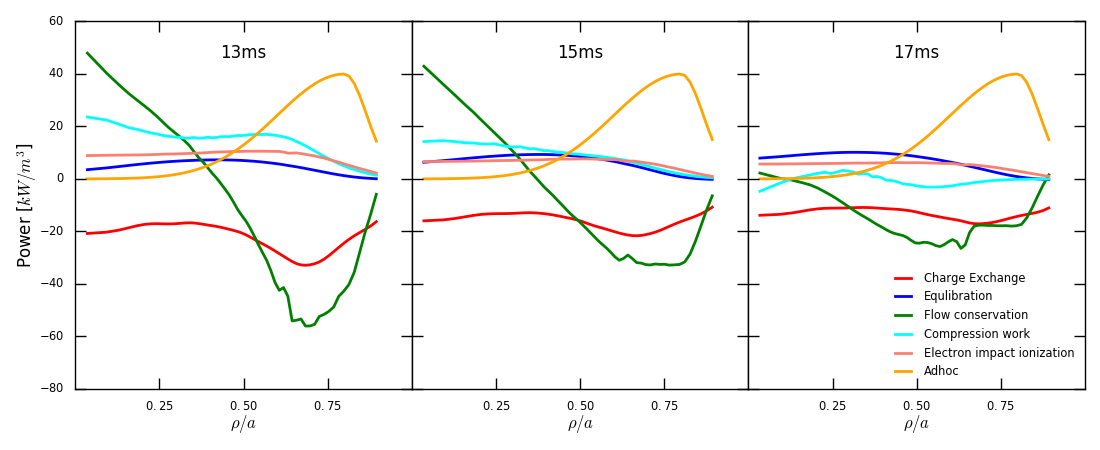
\includegraphics[width = \textwidth]{ion_transport_results/power_terms_with_adhoc.png}
    \caption[Power terms resulting from radial ion flow]{Power terms resulting from radial ion flow. Classical conduction have been omitted as it is of lower magnitudes than the plotted terms.}
    \label{fig:power_terms_with_adhoc}
\end{figure}


%TODO: There should be a paragraph on estimating the ion thermal confinement time that I'm not quite ready to write yet. 

From this model, the ion thermal confinement time can be estimated. The common definition of thermal confinement time is written as follows,
\begin{align}
    \tau_E &= \frac{W}{P_{\text{loss}}}\\
    &= \frac{W}{\partialt W - P_{\text{ohm}}}
\end{align}
However, in the context of the model, where the loss terms are known explicitly, it is more appropriate to specify $P_{\text{loss}}$ directly. In particular, 
\begin{align}
    P_{\text{loss}} &= - [P_{\text{CX}} + P_{\text{cond}} + P_{\text{flow cons}}]
\end{align}
The other terms in the model, including compressional work, \adhoc heating, and e-i equilibration heating, are considered power inputs, and thus do not factor into the calculation of the thermal confinement time. 
 % I don't think that these terms are 'external' to the plasma the way Ohmic heating or RF heating are external inputs to the plasma. By they are power inputs to the ion fluid rather than losses.
 %Edited -Xing
This means that for the consideration of this calculation, the flow terms as specified in section \ref{sec:flow_effects} are separated into the compressional heating part ($P_{\text{comp work}}$) which is not part of $P_{\text{loss}}$, and the flow conservation part ($P_{\text{flow cons}}$) which is. The confinement time of the model is shown in figure \ref{fig:conf_time}. It should be noted that this is not a direct measurement of the ion confinement time, but rather it is the ion confinement of a model that can be matched to observed temperature evolution.
\begin{figure}
    \centering
    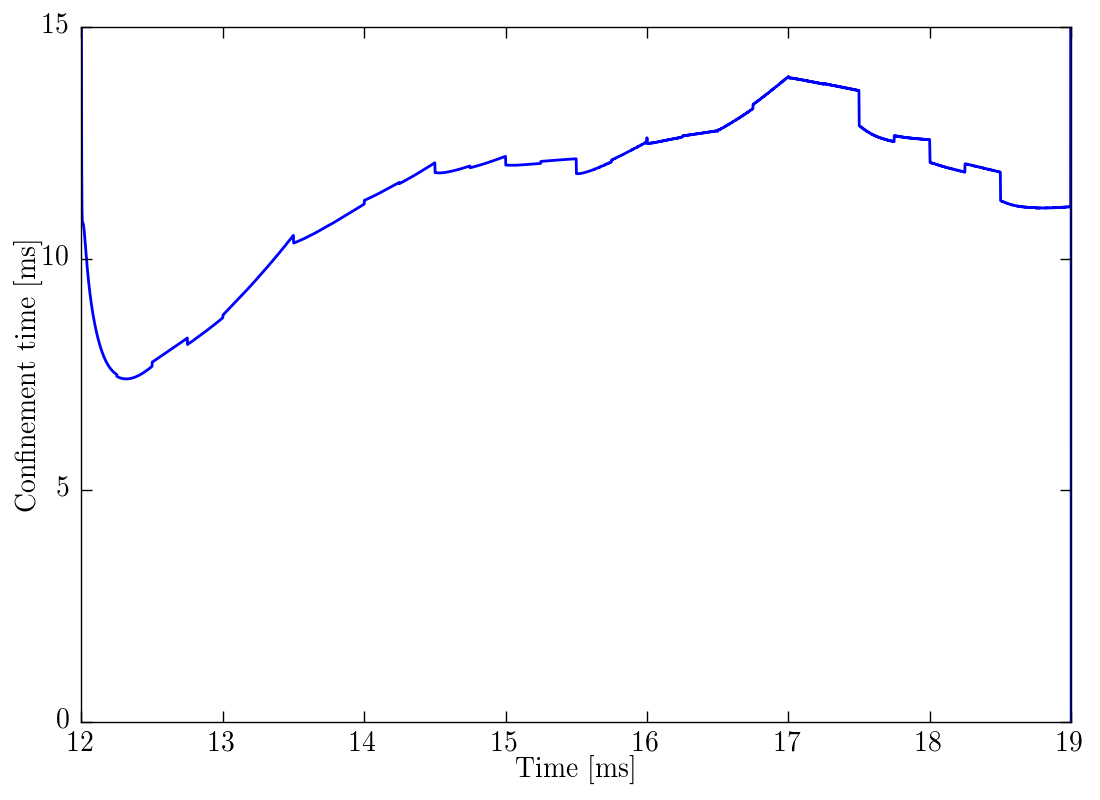
\includegraphics[width = \linewidth]{ion_transport_results/conf_time.png}
    \caption[Model ion confinement time]{Ion confinement of the model. It is calculated to be around 12ms for the 'main' part of PPCD (~15ms to the end of PPCD). The confinement time is poorer during onset of PPCD (< 15ms) but displays a roughly upward trend. The effect on temperature of this relatively poorer confinement is mitigated by the compressional heating active during the early period. }
    \label{fig:conf_time}
\end{figure}
The thermal confinement time is comparable to electron confinement time in PPCD calculated at ~ 10ms \cite{Chapman2001}, but it is not evident that the two are linked through physical mechanisms. Considering the decoupling of ion and electron temperature, it may be a coincidence that their confinement time seems to match. The model's confinement time further changes if the model temperatures are allowed to drift below the observed temperature by omitting the \adhoc heating term. In that case, the confinement time noticeably increase as the edge ion temperature decreases which decreases the heat loss due to outward particle flux in the edge, as well as somewhat reducing the charge exchange loss the the same region. 
%%% Now that you have calculated the ion thermal confinement time, how does it compare with other relevant time scales? For instance, how does it compare with the electron thermal confinement time for PPCD or standard plasmas? Are the results what you would expect or are they surprising?
%Elaborated. --Xing

\subsection{Profile and extent of \adhoc heating in the gradient regions}\label{sec:anomalous_heating}

The previous section glossed over the shape and location of the \textit{ad hoc} heating term used in order to present the results. However, there are comments to be made that would be of interest to readers. The driving determinant of the \textit{ad hoc} term is to enable the model to match the observations, but that does not mean that it is entirely free of physics considerations. The profile settled upon is an asymmetrical Gaussian (in $\rho_v$) made from two half Gaussian profiles with differing width. The profile peaks at $\rho_v/a = 0.75$, the approximate location of the reversal surface (see figure \ref{fig:q_profile}). The reversal surface is not only the home of all m = 0 modes, but also near tightly packed m =1 rational surfaces. Additionally, the peak and the width of the \textit{ad hoc} heating term is approximately coincident with the $T_e$ gradient region as measured via Thomson scattering. The edge half of the Gaussian shape have a smaller width to account for the fact that the turbulence that likely drives anomalous heating would be rapidly decreasing near MST's conducting shell, together with rapidly decreasing availability of free energy as temperature and density drops in the very edge. However, the modeling work and the CHERS measurements provide nearly no constraint on the very edge of the plasma. 
\begin{figure}
    \centering
    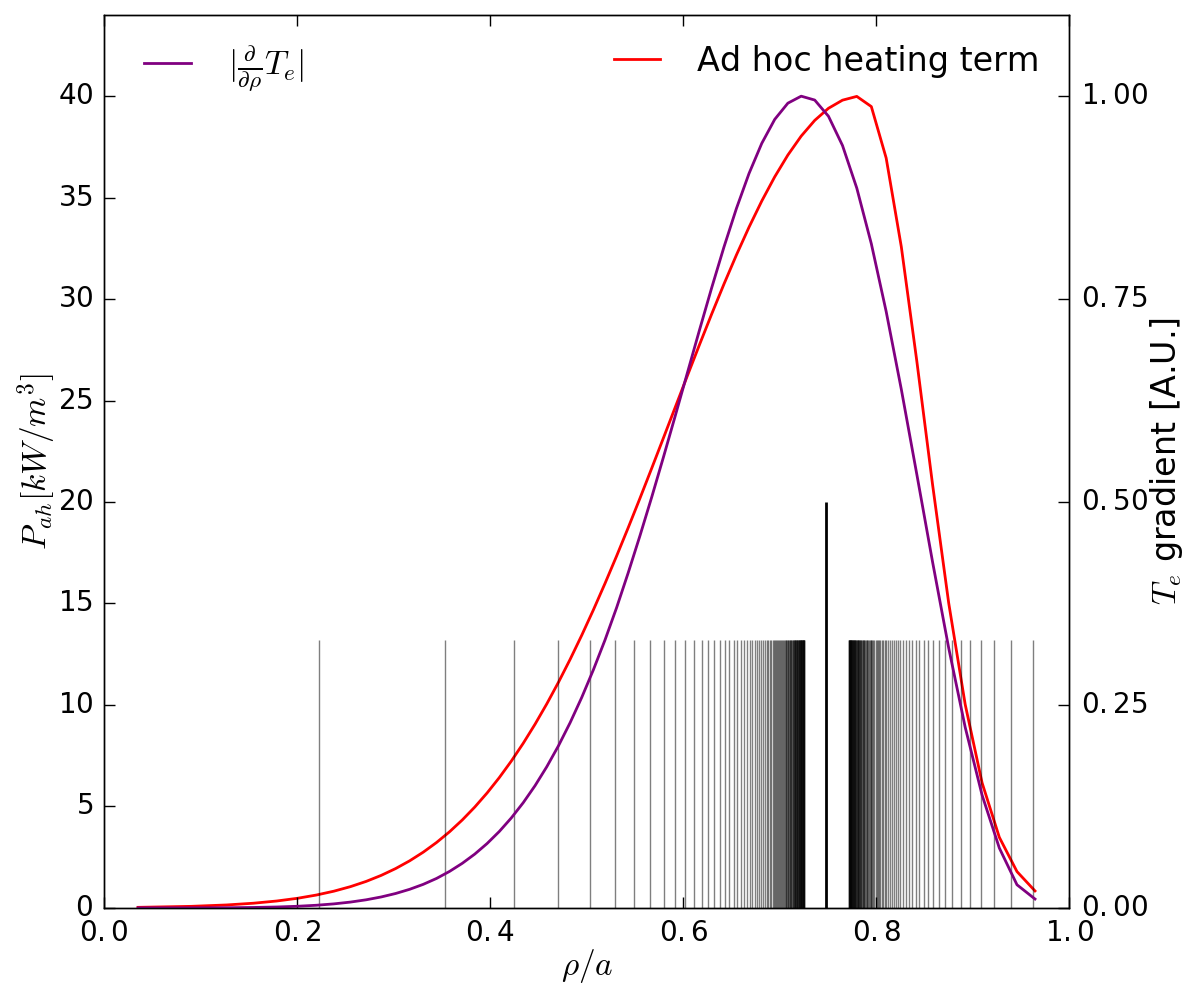
\includegraphics[width = \textwidth]{ion_transport_results/adhoc_profile.png}
    \caption[\textit{ad hoc} heating profile]{\textit{ad hoc} heating profile compared to normalized $T_e$  gradient. The long vertical line at $\rho/a \approx 0.75$ marks the location of the reversal surface, and the shorter lines marks out the resonant surfaces beginning with inner most the (1,6) surface. For a plot of the q profile associated, see figure \ref{fig:q_profile}.}
    \label{fig:ad_hoc_v_gradient}
\end{figure}
%Mark comments here:
%In addition to mentioning the edge localization, you should note that there are several sources of free energy that could drive heating mechanisms. First, there is residual tearing mode activity in PPCD plasmas that, while much lower in amplitude, still result in stochasticization of the magnetic field near the reversal surface. In addition, we are actively driving a current in the edge and may be affecting the current gradient in such a way that it can excite the edge-resonant modes. Finally, there is the edge density gradient which drives drift wave instabilities that give rise to turbulent electrostatic fluctuations.

%These are all free sources of energy that could provide sufficient energy for the modest amount of edge-localized ion heating your model suggests. This energy could be tapped through processes like turbulent damping of Alfven-waves through cyclotron resonance, stochastic heating due to the residual tearing modes near the reversal surface, driving edge-resonant tearing through the PPCD pulses, and turbulent heating which can channel heat from the electrons to the ions.
 
%For the last process, I started with Gennady’s paper and potentially made a mistake. For Gennady’s argument to be self-consistent the perpendicular diffusion process has to be separate from the process generating the electric field fluctuations. Otherwise, there is a problem with making the process irreversible.

%A more natural way of formulating the heating mechanisms available through drift wave turbulence is to consider ion Landau damping and frictional heating associated with zonal flow generation by the turbulence. A paper which lays these mechanisms out is here:
There are several mechanisms that may be responsible for this \adhoc heating, including cyclotron resonance heating from Alfven waves and stochastic heating from residual tearing modes activities near the reversal surface. Further, plasma turbulence such as driftwaves and zonal flow, both recently observed for PPCDs in MST\cite{Nishizawa2018, Nishizawa2019}, drives both quisilinear and nonlinear turbulent heating and enables the collisionless transfer of energy from electrons to ions through such mechanisms such as Landau damping of wave energy, and frictional heating via zonal flow. The volume integrated \adhoc heating used in the model is $\approx 144 kW$, which is small in the overall energy balance of the RFP. For example, the total magnetic energy ($ = \frac{B^2}{2\mu_0}$) goes from $\approx 275kJ$ to $\approx 300kJ$ and back during a typical period of analysis (spans 8ms from 12ms to 20ms). Thus a seemingly small transfer of energy from electrons or the magnetic equilibrium may be sufficient to account for the \adhoc heating added to model calculations.

More generally, the location and the width of the \textit{ad hoc} heating term roughly corresponds with the location of the $T_e$ gradient region (see figure \ref{fig:ad_hoc_v_gradient}). While electron gradients are not directly connected to ion thermal heating, they are sources of free energy driving turbulence that would generate heating. 

\subsection{Anomalous Transport vs. heating}

The \textit{ad hoc} heating term needed for the model can correspond to anomalous transport or heating, as the model does not account for stochastic transport mechanisms, or turbulent heating mechanisms. However, given the model's ability to predict the core temperature well even in the absence of the \textit{ad hoc} term, it is more likely that the discrepancy in the edge is accounted for by anomalous heating. 
Consider stochastic transport of heat, the stochastic counterpart to classical thermal conduction. The stochasticity increases the characteristic step size of the particle beyond the gyro-radius, and ions wondering along the stochastic field would collide another and exchange place' with it, transporting heat from the hotter location to the colder. Note that this is a purpose effort to separate the stochastic heat conduction/transport from the stochastic particle transport, as the particle transport and flux is indirectly included in the model (see the discussion in section \ref{sec:stochastic_effects}). The total \adhoc term needed in the model integrates to about 140kW over the volume of the plasma. If the \adhoc term is 'caused' by a anomalous transport mechanism, then the transport mechanism would be taking the thermal energy from hotter regions (\textit{ie.} core). For an estimation, one can assume that such a transport mechanism takes heat from the core region defined by $\rho/a \leq 0.4$ and deposit at $0.4 \leq \rho/a \leq 0.9$ (refer to figure \ref{fig:ad_hoc_v_gradient}). Thus defined, the core region have a volume of $\approx 1.25 m^2$, and lose heat at $~110kW/m^2$ making it the most significant term in the core. Further assuming a nominal core density of $0.7 \times 10^{19}/m^3$, the core cooling implied by such a transport would be $\approx 100eV/ms$ in addition to what the model currently predicts. This is significantly larger core cooling than the observations would allow (refer to figure \ref{fig:temperature_results_ah}).

While it cannot be ruled out that the \adhoc term in the model is the result of a combination of a anomalous transport mechanism, and a (relatively) radially uniform anomalous heating mechanism, it is very unlikely to be the effect of a anomalous transport mechanism only. To the first order, the result point to an anomalous heating mechanism active in the $T_e$ gradient region.

\subsection{Additional comments on thermal transport}

\begin{figure}
    \centering
    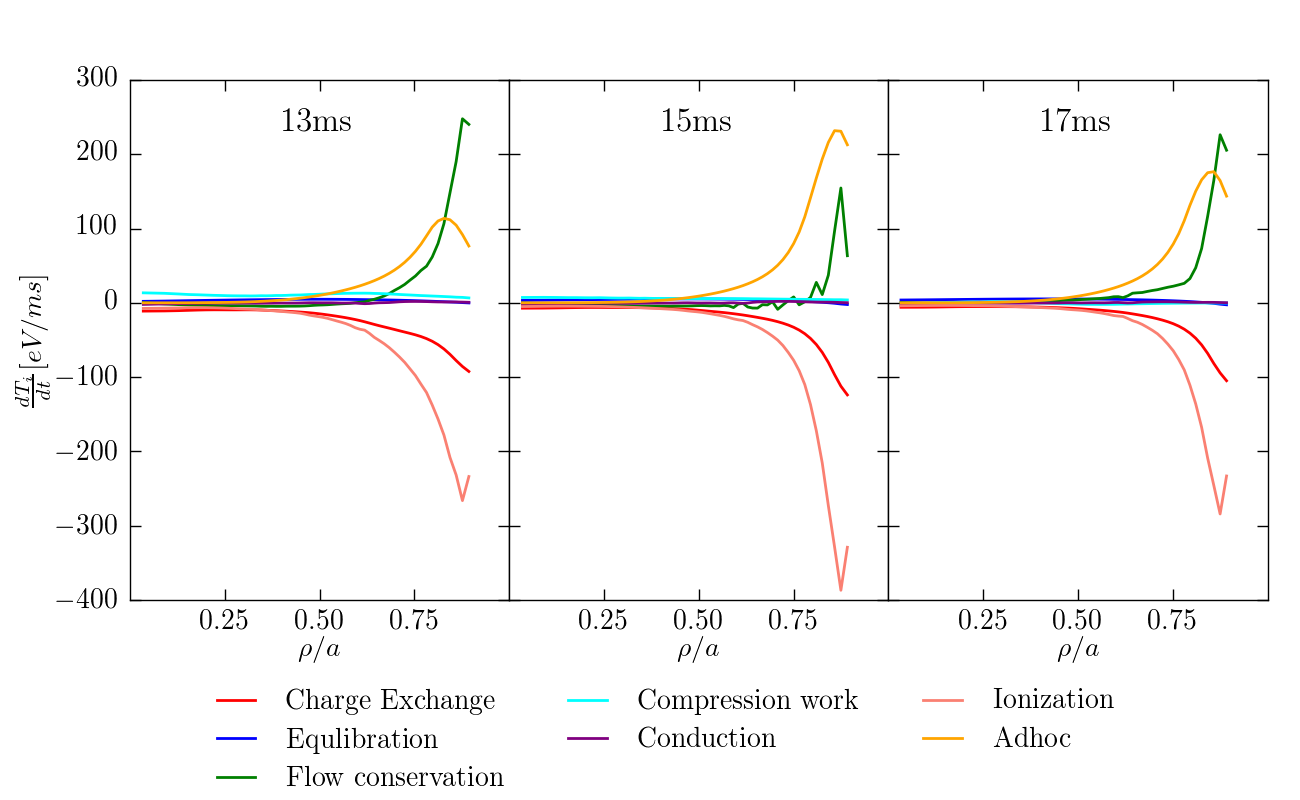
\includegraphics[width = \linewidth]{ion_transport_results/dtempdt_with_adhoc.png}
    \caption[$\partialt T_i$ due to various terms]{$\partialt T_i$ due to various terms in the model. The significance of this plot is explored more in the text. }
    \label{fig:temperature_change}
\end{figure}

\begin{figure}
    \centering
    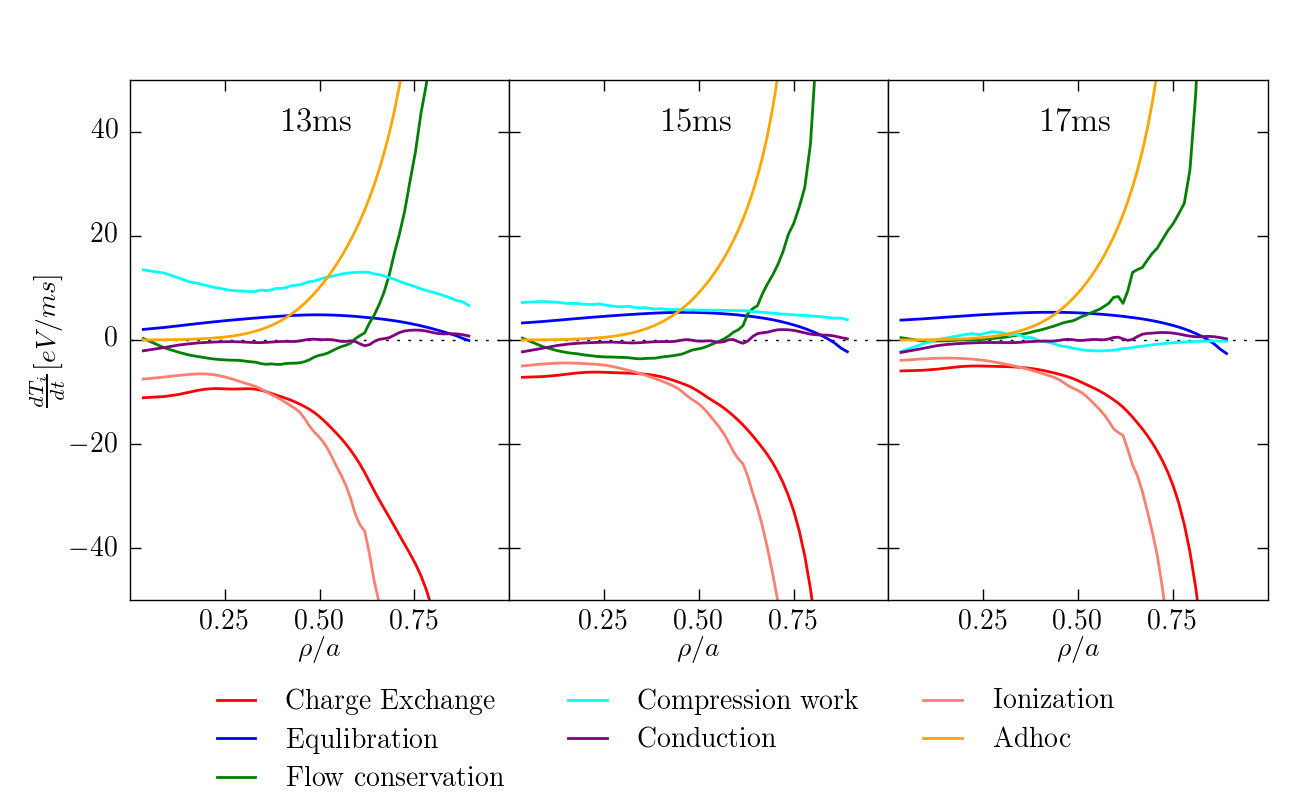
\includegraphics[width = \linewidth]{ion_transport_results/dtempdt_zoomed.png}
    \caption[$\partialt T_i$ core details]{$\partialt T_i$ due to various terms in the model, zoomed in to show the core dynamics clearer. Note the disappearing effect of compressional work. }
    \label{fig:temperature_change_zoomed}
\end{figure}

It is instructive to look at the modeled terms from the point of view of their contribution to $\partial T_i /\partial t$ (figure \ref{fig:temperature_change} and figure \ref{fig:temperature_change_zoomed}). There is two effects worth noting. The first is that some power terms do not have the same effect on temperature as thermal energy. As mentioned before, $P_{\textrm{ionization}}$ which represents the energy 'recovered' from the warm neutral population through re-ionization, reduces the ion temperature despite being a positive power term. This is due to the fact that it brings cooler particles into to the ion fluid. The cooling effect of ionization is the most significant in the edge region, but important throughout the plasma volume. Conversely, the flow effects are (aside from the \textit{ad hoc} term) the most significant for increasing the temperature, due to the flow of hotter ions to the cooler edge. But at the same time, it competes with charge exchange for being the significant energy loss term. The second is that the $P_{\textit{ad hoc}}$ contribution to $\partial T_i / \partial t$ is modified by density, causing it to chage despite the power remaining constant. Especially, it's peak is farther out in the edge as compared to that of $P_{\textit{ad hoc}}$ itself. Looking at figure \ref{fig:temperature_change_zoomed}, we can see that \textit{ad hoc} term's contribution to $\partial T/\partial t$ is relatively constant inside $\rho/a = 0.75$. The response outside of this location (\textit{i.e.} the outside half-Gaussian of the \textit{ad hoc} profile) changes significantly. Though the model is not well constrained here, as the outer most CHERS measurement is at $\rho/a = 0.75$. If the \textit{ad hoc} heating is indeed related to the stochastic mechanism as detailed by G. Fiksel, the $\left.\partial T_{i}/\partial t\right|_{\textit{ad hoc}}$ would be relatively constant and the resultant power would change as density changed. 

The e-i equilibration term is generally weak, resulting in the temperature separation seen in PPCD plasmas. Extrapolating to typical reactor densities, however, would imply that the equilibration heating would in crease by ~ 2 order of magnitude (both $n_e$ and $n_i$ would increase by an order of magnitude) while the biggest core loss term, charge exchange, would increase less as the neutral sourcing will increase will plasma density, but the neutral penetration will decrease correspondingly. As is currently, the charge exchange loss and the net flow loss (aka particle loss) are the two main loss mechanisms. Efforts to limit neutrals in the plasma may be beneficial, but high density and temperature plasmas, the neutrals are likely to have a much reduced role. Net ion particle loss will likely be the dominant challenge to RFP ion confinement in PPCD-like conditions. 



\section{Summary}

Experimental results show the 1-D ion thermal transport model adequately predicts the ion temperature evolution in the core, but needs an \adhoc term in the gradient region to match observations there. Of particular importance to the model is the neutral dynamics as calculated via the Monte-Carlo simulation code DEGAS2. This simulation is important in calculating the charge exchange loss from the core. The results indicates that the neutral population in the core is 'warm' and the charge exchange loss is somewhat hollow. The ionization of neutrals are found to 'recover' some of the energy lost to the neutral fluid, but this results in decrease in temperature. The source rate geometry and continuity equations calculations finds that PPCD plasmas under goes an inward pinch during the first milliseconds, which contributes to core temperature via compression. However, the net particle flux at the edge is outwards and represents a significant loss term. When compared to ion temperature measurements, the model is found to be unable to match the observation in the gradient region unless an radially local \adhoc heating term is added. Comparisons are drawn between the \adhoc term needed and estimates of fluctuation induced heating and found to be plausible.


\printbibliography
\end{refsection}